\documentclass[12pt,english]{article}
\usepackage{preamble}
\newcommand{\macrotikz}{\documentclass[tikz]{standalone}
\usepackage{tikz}
\usepackage{pgfplots}
\pgfplotsset{compat=newest}
\usetikzlibrary{plotmarks}
\usetikzlibrary{arrows.meta}
\usepgfplotslibrary{patchplots}
\usepackage{grffile}
}

\begin{document}
\cleardoublepage
\pagenumbering{gobble}
%%%%%%%%%%%%%%%%%%%%%%%%%%%%%%%%%%%%%%%%%
% University Assignment Title Page 
% LaTeX Template
% Version 1.0 (27/12/12)
%
% This template has been downloaded from:
% http://www.LaTeXTemplates.com
%
% Original author:
% WikiBooks (http://en.wikibooks.org/wiki/LaTeX/Title_Creation)
%
% License:
% CC BY-NC-SA 3.0 (http://creativecommons.org/licenses/by-nc-sa/3.0/)
% 
% Instructions for using this template:
% This title page is capable of being compiled as is. This is not useful for 
% including it in another document. To do this, you have two options: 
%
% 1) Copy/paste everything between \begin{document} and \end{document} 
% starting at \begin{titlepage} and paste this into another LaTeX file where you 
% want your title page.
% OR
% 2) Remove everything outside the \begin{titlepage} and \end{titlepage} and 
% move this file to the same directory as the LaTeX file you wish to add it to. 
% Then add \input{./title_page_1.tex} to your LaTeX file where you want your
% title page.
%
%%%%%%%%%%%%%%%%%%%%%%%%%%%%%%%%%%%%%%%%%
%\title{Title page with logo}
%----------------------------------------------------------------------------------------
%   PACKAGES AND OTHER DOCUMENT CONFIGURATIONS
%----------------------------------------------------------------------------------------


\begin{titlepage}

\newcommand{\HRule}{\rule{\linewidth}{0.5mm}} % Defines a new command for the horizontal lines, change thickness here

\center % Center everything on the page

%----------------------------------------------------------------------------------------
%   LOGO SECTION
%----------------------------------------------------------------------------------------

\includegraphics[width=\textwidth]{fig/Logos}\\[2cm] % Include a department/university logo - this will require the graphicx package
 
%----------------------------------------------------------------------------------------
%   HEADING SECTIONS
%----------------------------------------------------------------------------------------

\textsc{\LARGE Brussels Faculty of Engineering}\\[1.5cm] % Name of your university/college
\textsc{\Large Modulation \& Coding}\\[0.5cm] % Major heading such as course name
\textsc{\large ELEC--H401}\\[0.5cm] % Minor heading such as course title

%----------------------------------------------------------------------------------------
%   TITLE SECTION
%----------------------------------------------------------------------------------------

\HRule \\[0.4cm]
{ \huge \bfseries Simulation of a DVB--S2 Communication Chain}\\[0.4cm] % Title of your document
\HRule \\[1.5cm]
 
%----------------------------------------------------------------------------------------
%   AUTHOR SECTION
%----------------------------------------------------------------------------------------

% If you don't want a supervisor, uncomment the two lines below and remove the section above
\Large \emph{Authors:}\\
Cédric~\textsc{Hannotier} \\% Your name
Badr-Ali~\textsc{Mouaden} \\
Mahtieu~\textsc{Petitjean}\\[2.5cm] % Your name

%----------------------------------------------------------------------------------------
%   DATE SECTION
%----------------------------------------------------------------------------------------

{\large \today}\\[2cm] % Date, change the \today to a set date if you want to be precise


%----------------------------------------------------------------------------------------

\vfill % Fill the rest of the page with whitespace

\end{titlepage}



\tableofcontents

\newpage
\cleardoublepage
\pagenumbering{arabic}

\section{Introduction}
This report presents the simulation of a DVB-S2 communication chain. The most important design parameters were varied in order to illustrate their impact on the quality of the communication via the bit error rate (BER).

This project was divided in three steps. Each of these steps is presented, then various graphs illustrate the important concepts and results. To conclude each section, questions regarding the simulation and the communication chain itself are answered.

\section{Optimal communication chain over the ideal channel}\label{sec:step1}
\subsection{Simulation}

The implementation scheme is shown in Figure \ref{fig:block}.

\begin{figure}[H]
    \centering
    \includegraphics[width = .9\textwidth]{fig/block.png}
    \caption{Block scheme of the ideal channel}
    \label{fig:block}
\end{figure}

The various components of the communication chain are detailed hereafter. The channel encoder is not yet implemented, and the symbols mapping/demapping were provided.

\subsubsection{Halfroot Nyquist filter}

After the mapping, the complex symbols are convolved with a root raised-cosine filter. It allows to limit the communication bandwidth, as illustrated in Figure \ref{fig:filter} where the PSD of the symbol stream are shown before and after filtering, with a rolloff factor $\beta$ of $0.3$. The symbol frequency was fixed to 2 \si{\mega \hertz}, which translates to a cutoff frequency of 1 \si{\mega \hertz}.

\begin{figure}[H]
\centering
    \includegraphics{fig/filter.tex}
     \caption{PSD of the symbol stream at the transmitter before and after filtering}
    \label{fig:filter}
\end{figure}

At the receiver side, the stream is convolved again with the matched filter, forming a Nyquist filter and maximizing the SNR. The Nyquist filter allows to cancel the ISI in the sense that it reduces to a Dirac pulse when sampled at the symbol frequency, as shown in Figure \ref{fig:isi}. Hence, no symbol of the symbol stream overlaps with the current received symbol.

\begin{figure}[H]
\centering
    \includegraphics{fig/isi.tex}
     \caption{Illustration of the cancellation of ISI by the Nyquist halfroot filter}
    \label{fig:isi}
\end{figure}


\subsubsection{Noise addition}

The channel is corrupted by Additive White Gaussian Noise (AWGN), which is simulated using its baseband equivalent representation. The channel was simulated for various SNR (defined with respect to the bit energy) and various modulation schemes, and the results are plotted in Figure \ref{fig:ber}. The simulations confirm the theoretical results.


\begin{figure}[H]
\centering
    \includegraphics{fig/ber2.tex}
    \caption{Bit error rate as a function of the SNR for various modulations. The full lines correspond to the theoretical curves and the dots to the simulation.}
    \label{fig:ber}
\end{figure}

As expected, more energy is required to have the same BER when the constellation size is increased. It is worth noting that the worst BER value that could be achieved is 0.5, corresponding to a random choice of the binary values. Moreover, the BER curves for 2-PAM and 4-QAM are superposed because a 4-QAM modulation can be seen as two 2-PAM modulations in quadrature.



\newpage
\subsection{Questions}

\subsubsection{Questions regarding the simulation}

\paragraph{It is proposed to use the baseband equivalent model of the AWGN channel. Would it be possible to live with a bandpass implementation of the system ?} \mbox{}

The baseband model allows to implement the simulations regardless of the carrier frequency. If the system were simulated in bandpass, the required sampling frequency would be extremely high and unrealistic.

\paragraph{How do you choose the sample rate in Matlab ?} \mbox{}

The sampling rate should be at least twice as high as the symbol frequency. It will be increased further when simulating the sample time shift in the third step.

\paragraph{How do you make sure you simulated the desired $E_b/N_0$ ratio ?} \mbox{}

First the energy of a bit is evaluated, then the noise power is computed in order to obtain the desired $E_b/N_0$ ratio. The energy of the bit $E_b$ is given by

\begin{equation*}
    E_b = \frac{T_{samp}}{2 N_{bits}} \sum_{n} {\left| s \left[ n \right] \right|}^2
\end{equation*}

Then $N_0$ can be chosen according to the wanted SNR and the noise is added to the symbols using the baseband representation :

\begin{equation*}
    r \left[ k \right] = \sqrt{N_0 f_{samp}} \left\{ \mathcal{N}(0,1) + j \mathcal{N}(0,1) \right\}  
\end{equation*}

The square root is present because of the baseband representation of the noise. Indeed, the computed power is equally distributed between the real and imaginary parts of the noise.

\paragraph{How do you choose the number of transmitted data packets and their length ?} \mbox{}

A rule of thumb is to send $10^{n+2}$ bits of data in order to reliably observe of BER of $10^{-n}$ as it corresponds to 100 detected errors. Moreover, the total number of bits should be a multiple of the number of bits per symbol used in the modulation scheme. The Figure \ref{fig:ber} was realised by sending around $10^8$ bits of data.

\subsubsection{Questions regarding the communication system}

\paragraph{Determine the supported (uncoded) bit rate as a function of the physical bandwidth.} \mbox{}

The bit rate $R$ is given by $R = \frac{log_2 (M)}{T}$ where $M$ is the number of symbols and $T$ is the symbol duration. The Nyquist filtering yields a relationship between the symbol duration and the bandwidth, $\Delta f = 2/T$ (this can be seen on Figure \ref{fig:filter} where T = 0.5 \si{\micro \second} and $\Delta f = 2$ \si{\mega \hertz}). This gives:

\begin{equation*}
    R = \frac{log_2 (M) \ \Delta f}{2}
\end{equation*}

\paragraph{Explain the trade-off communication capacity/reliability achieved by varying the constellation size.} \mbox{}

As detailed in the previous question, increasing the constellation size (the number of bits transmitted per symbol $M$) allows to increase the bit rate. However, the minimum euclidean distance between the symbols in the constellation size decreases, which causes the error probability to increase. As a result, to achieve a similar BER, more energy is required when the constellation size increases but the bit rate also increases.

\paragraph{Why do we choose the halfroot Nyquist filter to shape the complex symbols ?} \mbox{}

The halfroot Nyquist filter allows to limit the communication bandwidth (it is more spectrally efficient than the plain rectangular window) and allows to cancel ISI.

\paragraph{How do we implement the optimal demodulator? Give the optimization criterion.} \mbox{}

The optimal demodulator is implemented 	as a bank of K filters matched to the basis functions of the modulation scheme: 

\begin{equation*}
	h_i(t) := s_i(-t) \hspace{1cm}  i=1,...,K
\end{equation*}

The outputs to such filters are the autocorrelations between the input signal and the basis functions. The filters are mathematically equivalent to a bank of K correlators. The optimisation criterion is the maximisation of the SNR at the output. It is realized by the matched filters, and the SNR will be equal to $\frac{2\mathcal{E}}{N_0}$.

\paragraph{How do we implement the optimal detector? Give the optimization criterion.} \mbox{}

There exist two possible optimization criteria for the detector. First, the maximum a posteriori (MAP) criterion, which minimises the error probability by exploiting the knowledge of the a priori probabilities $p(\underline{s}_m)$ and the conditional probabilities $p(\underline{r}|\underline{s}_m)$, where $\underline{r}$ is the observation. It selects the symbol which is the most likely to have been sent, knowing that we observed $\underline{r}$.
	
	\begin{equation*}
		\underline{\tilde{s}}^{\text{MAP}}_m = \underset{\underline{s}_m}{\text{max}} \ p(\underline{s}_m |\underline{r}) \stackrel{\text{Bayes}}{=}
		\underset{\underline{s}_m}{\text{max}} \ p(\underline{r} |\underline{s}_m) p(\underline{s}_m)
	\end{equation*}
	
The maximum likelihood criterion is equivalent to the MAP criterion when all the M symbols are equally probable, so that $p(\underline{s}_m) = 1/M$ is constant and can be dropped when maximizing the probabilities.
	
	\begin{equation*}
		\underline{\tilde{s}}^{\text{ML}}_m = \underset{\underline{s}_m}{\text{max}} \ p(\underline{r} |\underline{s}_m) 
	\end{equation*}
	
The ML criterion determines what symbol is the most likely to have produced the received signal by selecting the symbol which has the lowest euclidean distance to the received symbol.



\section{Low-density parity check code}
\subsection{Simulation}

The channel encoder that was skipped in section \ref{sec:step1} is now implemented as a low-density parity check code (LDPC) encoder. Soft and hard decoding have been implemented with a code rate of 1/2 and their performance is compared next.

The channel coding adds structured redundancy  to the information sent by the transmitter to be able to detect and correct errors at the receiver side. The LDPC code has the property that the check matrix is sparse, allowing a lower complexity of the implementation.

\subsubsection{Hard decoding}
\iffalse
\begin{figure}[H]
\centering
    \includegraphics{fig/HardLDPC.tex}
     \caption{Hard LDPC}
    \label{fig:HardLDPC}
\end{figure}
\fi

The hard decoding is based on the implementation of a Tanner graph. The influence of the maximal number of iterations on the BER curves is shown in Figure \ref{fig:HardLDPCbis} for a 16-QAM modulation. The conclusions can be generalized to any modulation.

\begin{figure}[H]
\centering
    \includegraphics[width=\textwidth]{fig/HardLDPCbis.tex}
     \caption{Effect on the BER curves of Hard LDPC decoding for a 16-QAM modulation}
    \label{fig:HardLDPCbis}
\end{figure}

For the hard decoding, the performance is worsened at low SNR. Indeed, a noise which is too important causes the code to add errors when it is trying to correct them. Increasing the maximal number of iterations allows a slight improvement in performance.

\subsubsection{Soft decoding}

In practice, hard decoding is never used as the soft decoding allows for much better performance. Instead on basing the decision on the received bits, it computes probablities based on the received symbols. The results of the simulations for a 2-PAM is shown in Figure \ref{fig:SoftLDPC}.

\begin{figure}[H]
\centering
    \includegraphics{fig/SoftLDPC.tex}
     \caption{Effect on the BER curves of Hard LDPC decoding for a 16-QAM modulation}
    \label{fig:SoftLDPC}
\end{figure}

The theoretical curve for the ideal communication chain as well as the curve for hard decoding are shown as references. The improvement is significant with soft decoding.

\subsection{Questions}

\subsubsection{Questions regarding the simulation}

\paragraph{When building the new BER curves, do you consider the uncoded or coded bit energy on	the x-axis?} \mbox{}

The coded bit energy is considered here.

\paragraph{How do you limit the number of decoder iterations?} \mbox{}

For the hard decoding, the iterations stop either when the maximum number of iterations is reached or when the syndrome is zero.

For the soft decoding,  stop either when the maximum number of iterations is reached or when there is no more detected errors.

\paragraph{Why is it much simpler to implement the soft decoder for BPSK or QPSK than for 16-QAM or 64-QAM?} \mbox{}

In the case of the 16-QAM or 64-QAM, the euclidean distance should be computed when decoding. This is not the case for BPSK and QPSK, where the decision can be made only by looking at the real and imaginary part of the received symbols.

\subsubsection{Questions regarding the communication system}

\paragraph{Demonstrate analytically that the parity check matrix is easily deduced from the generator matrix when the code is systematic.} \mbox{}

A code is systematic when the mapping is such that part of the code vector coincides with the message vector. In that case, the generator matrix has the form $\underline{\underline{G}} = \left[\underline{\underline{P}} | \underline{\underline{I}}\right]$, with $\underline{\underline{P}}$ the parity array and $\underline{\underline{I}}$ the identity matrix of the corresponding size.
The parity check matrix should be created so that its rows are orthogonal to the rows of the generator matrix:

\begin{equation*}
 \underline{\underline{G}} \cdot \underline{\underline{H}}^T = \underline{\underline{0}}
\end{equation*}

The solution to this equation is given by $\underline{\underline{H}} = \left[\underline{\underline{I}} | \underline{\underline{P}}^T\right]$. Indeed:

\begin{equation*}
	\underline{\underline{G}} \cdot \underline{\underline{H}}^T = \left[\underline{\underline{P}} | \underline{\underline{I}}\right] \cdot \left[\underline{\underline{I}} | \underline{\underline{P}}^T\right]^T =  \underline{\underline{P}} \oplus  \underline{\underline{P}} =0
\end{equation*}

\paragraph{Explain why we can apply linear combinations on the rows of the parity check matrix to produce an equivalent systematic code.} \mbox{}

The rows of the parity check matrix are the basis vectors of a subspace which is perpendicular to the subspace spanned by the generator matrix. A linear combination of these basis vectors will still be a basis for the same subspace and the resulting code will be equivalent.

\paragraph{Why is it especially important to have a sparse parity check matrix (even more important	than having a sparse generator matrix)?} \mbox{}

A sparse parity check matrix allows to significantly reduce the complexity of the decoder. Indeed, element $H_{ij}$ being equal to 1 results in a logical connection in the Tanner graph between the check-node $c_i$ and the variable-node $v_j$. Hence, reducing the number of 1's in $\underline{\underline{H}}$ reduces the number of exchanged messages and the number of computations.

\paragraph{Explain why the check nodes only use the information received from the other variable nodes when they reply to a variable node.} \mbox{}

The information exchanged between the check and variable nodes has to be statistically independent for hard and soft decoding. This means that only the information which is not related to the current node is used to compute the answer.

\section{Time and frequency synchronisation}
\subsection{Simulation}
In this section, the synchronisation errors caused by the hardware, the carrier phase and frequency shift are simulated, then algorithms allowing to reduce them are introduced.

\subsubsection{Synchronisation errors}

On \autoref{fig:CFOphi} is shown how the CFO affects the constellation. The linearly increasing phase shift caused by the CFO causes a rotation of the symbols. This effect is first manually corrected to study the impact of ISI only.

\begin{figure}[H]
    \centering
    % This file was created by matlab2tikz.
%
%The latest updates can be retrieved from
%  http://www.mathworks.com/matlabcentral/fileexchange/22022-matlab2tikz-matlab2tikz
%where you can also make suggestions and rate matlab2tikz.
%
\begin{tikzpicture}

\begin{axis}[%
width=.75\textwidth,
height=0.4\textheight,
at={(0.758in,0.481in)},
scale only axis,
xmin=-1.5,
xlabel=Real part,
ylabel=Imaginary Part,
xmax=1.5,
ymin=-1.5,
ymax=1.5,
axis background/.style={fill=white}
]

\addplot [only marks,  mark=*, mark options={solid, black}]
  table[row sep=crcr]{%
-0.275074360503006	0.031028842354905\\
-0.148889862565281	-0.0130985932651375\\
0.00538347175725273	-0.112627187948849\\
0.132958309159965	-0.0897330601530277\\
-0.0593837203887866	-0.00646170952355751\\
0.608440441657752	-0.603618839007926\\
-0.838993061665298	-0.606488888750607\\
0.772086158265415	-0.882233673433549\\
0.419961208155234	1.00962325000435\\
0.635282274042976	-0.813420882164765\\
0.299324252527225	0.949846021591672\\
0.522408763114605	-0.752309059126966\\
-1.07624617616603	0.502521280420278\\
-0.626305388418813	0.4919263234996\\
-0.983955710283295	1.06486739884716\\
-0.572790314565448	-0.826685756013168\\
-0.675692373399249	-0.72024995724919\\
-0.394848536115233	-0.840806526354487\\
-0.819918774666542	0.976541169146\\
0.59778373447911	0.488323455133767\\
-0.746503990186677	0.720741452671712\\
0.929964154568692	-0.89723498968404\\
0.655131136052147	0.765154903978667\\
-0.602883680809908	0.482950064824212\\
-0.751765421863797	0.837621216604283\\
0.552468816571611	0.905647450539323\\
-0.641115466711379	-0.991640624745691\\
-0.885587004770507	0.85774688408252\\
-0.791303731139457	-0.963530376858672\\
-0.743632562183174	-0.844645942803126\\
0.636123225927949	0.338441553204643\\
0.611213424875144	0.678150524602402\\
0.663078034096211	-0.503691760299607\\
-0.554596756552234	0.838421970663701\\
-0.555516302312948	0.518608866193063\\
0.24211805613983	0.758069271282409\\
0.813759522273116	0.608208482175125\\
-0.930374066729103	0.714042132922138\\
-0.603561220308552	0.751259434498267\\
-0.834089657642483	-0.778543332109609\\
0.566539912987205	0.642490644202337\\
0.502765749699848	0.875812204565474\\
-0.902264170307413	0.20012245681573\\
0.966963772046459	0.963727930171894\\
-0.806415064748563	-0.749905548507529\\
0.614221620421337	0.761314096492191\\
-1.0109066225647	0.410028577574734\\
0.764897201413298	1.05334581555584\\
-0.842773762723503	-0.755599685528135\\
-0.298634402705431	-0.723005256249798\\
-0.752017660169184	0.478962028234168\\
0.714437375308711	0.49770055917221\\
-0.805859167064012	-0.738345592543543\\
0.866118417911282	-0.804041268364328\\
-0.756684312115462	0.907151805250295\\
-0.729508678690953	0.2818366381849\\
0.688497753395228	0.857105852419397\\
-0.793196978088067	-0.868360384907852\\
-0.393904232528291	0.615036072994002\\
-0.640507998152296	0.460735248514807\\
-0.471275138210156	-0.625170170524948\\
-0.730162304095691	-0.80785423973491\\
0.677754252645761	0.583654535642871\\
-0.816127464594894	-0.861884713650333\\
1.05783328610077	-0.544710205714217\\
-0.680128028822793	-0.824392780864888\\
-0.69931533775715	-0.716952910568777\\
-0.672518427660595	-0.593593234381476\\
-0.66000889967851	-0.874309738964441\\
-0.801204651093342	0.606463162019251\\
-0.798892589077559	-0.643746088286139\\
0.988587206745426	-0.365199153622153\\
-0.878903352965184	0.721607077076557\\
0.784983198995423	-0.551203827357122\\
-0.879547589423843	-0.638086161673864\\
0.928549563380645	0.752130897454578\\
-0.459273476093769	-0.846468604298876\\
-0.809101138532701	0.450039620050903\\
0.68280164925093	0.525520431744708\\
-0.870189991159552	0.724384613541653\\
-0.546526720757448	0.662807840550096\\
0.858438439182964	0.551617979176084\\
-1.34763419646402	0.505429561921378\\
0.786003127124291	-0.627258794422121\\
-0.855525883691427	0.72125918754288\\
-0.65622089482161	0.769056695799189\\
0.581996286190266	-0.894158465990959\\
0.551481235100045	1.05716080711382\\
-0.127489243893464	-0.847661853715951\\
-0.883918837672668	0.631417804874411\\
0.848244073841558	0.74029180719841\\
-0.821754959275901	0.60221603942174\\
0.84539408076611	-0.603662260432429\\
-0.577501584368965	-0.611816390907839\\
-0.532305065421303	-0.731078468683418\\
0.882365516775026	0.886168882197693\\
-0.842669217208009	-0.941537462744276\\
0.809526578087723	0.761523941470908\\
-0.929673688311083	-0.851759369007869\\
0.985762533360854	-0.441698798651423\\
-1.03527948131454	0.515498598543433\\
1.16305519801648	-0.536613309335827\\
-0.684852346515902	-0.706401588665981\\
-0.743691268929236	0.588784571828406\\
-0.793498642958326	0.618158500719046\\
0.646140337870267	0.921252373743076\\
-0.747325774492686	0.470014902113425\\
0.758549101346552	0.711937701813479\\
0.710890251610011	-0.935732509794225\\
-1.04641371639677	0.802086185676997\\
0.743533057484136	0.541198487353323\\
-0.575905169173997	0.541622493828985\\
-0.818152254012363	0.512193528583056\\
-0.841365638160233	0.562056033798306\\
0.681973432058391	-0.700757558543083\\
0.550870492232959	1.37772272619954\\
0.601605285688333	0.641644052401027\\
0.54554293311023	0.862281955588389\\
-0.768801099671206	-0.704057756134916\\
-0.688289463308617	-0.403199436832222\\
0.670223784466907	0.959116003683079\\
-1.18724836220319	0.699588185415836\\
1.0108289444863	-0.59224832185536\\
-0.809225405735668	0.467618050662619\\
-0.765352674766321	0.653952822138635\\
-0.586840637939637	-0.790611759866254\\
-0.57751535623079	-0.912068429955476\\
-1.08200876234534	0.593563694904741\\
-0.493626833729214	-0.960180902792757\\
-0.743796525008694	-1.059033817548\\
0.64560638874364	-0.560248190689592\\
0.504596533354895	0.646626861631779\\
-0.403189610237981	-0.830970960815244\\
-0.600899918444077	0.637989748770013\\
-0.873755054645127	-0.963907527795709\\
0.680021678784904	-0.592014863953409\\
-0.885681680520171	-0.804070605488915\\
-0.507737855722277	-0.750246446219548\\
-0.942177750088007	0.571912836871726\\
0.446550768528435	0.951267041342452\\
-0.65503421126886	-0.565861215611999\\
-0.459855940459566	-1.0287706184308\\
0.603048458759636	1.01169136794544\\
1.05569945841658	-0.505613674202773\\
0.501018271979064	0.884308089691292\\
0.584387579570233	0.655972752831057\\
0.480934254089675	1.15698979941751\\
-0.354661249389624	-0.789939886269492\\
-0.732839864232141	-0.794321265312085\\
0.512933615818048	0.693729464473437\\
-0.843038949440359	0.530301926530008\\
-0.861231357142281	0.724175087425051\\
0.801757427619376	-0.823752901211319\\
-0.593373978214209	-0.971526976790504\\
-0.450838551775587	-0.870281382139237\\
-0.790295185902388	0.650389980850563\\
-0.428470125710408	-1.09253258151726\\
-0.753290124973672	0.376328723771649\\
0.668085725308391	0.629074433428171\\
0.165506070669052	0.951822679991209\\
0.885579018891207	-0.597025791787472\\
-0.299669964618198	-0.814682974158258\\
0.808435568574208	-0.646779647663678\\
0.69290160259123	-0.668250943127324\\
-0.85338923427621	0.708616988476596\\
-0.731736052039681	0.520602187720469\\
-0.540799276639686	-0.649666929949251\\
0.644943415144342	-0.191934804781235\\
-0.745413090752866	-0.667399415296412\\
-0.608016030772345	0.487394787868416\\
0.583319855302853	0.759598457377606\\
0.785732879677213	-0.607600013616746\\
0.603087328136722	0.738870209603549\\
0.890947118838872	-0.836279353525178\\
-0.585330781076752	-0.713938833429007\\
0.376571661831266	0.698991837836874\\
1.01947036555253	-1.07623788049103\\
-0.896666387280718	0.673792398187312\\
0.952396813442825	-0.424178875621712\\
0.405727895803617	1.15339081899502\\
-0.823006029315941	0.23190853280936\\
0.467160449654999	1.14061105350517\\
0.708037975496415	-0.586803904702824\\
0.386660079506713	0.950592112095999\\
0.888557896543201	-0.702411497193001\\
-0.853102281818469	0.973324181755163\\
-0.480705397054267	0.308905710080294\\
0.575180008330995	0.75995888440664\\
-0.781643868951168	-0.792257430000087\\
-0.521732946682391	-0.723419875566645\\
-0.65216009147344	-0.898736814351236\\
-0.397585758440143	-1.06503733696972\\
-0.644172288198801	-0.606268965281504\\
0.725957059993594	-0.296943952030993\\
-0.659315022505375	-0.75029242156842\\
-0.766617899507042	0.50446325281104\\
0.511885796797066	0.684282446479984\\
0.632540836075582	-0.580846419586762\\
-0.371072415344454	-0.771121117044887\\
-0.377745372931398	-0.602164782688964\\
-0.128469357461197	-0.657739360571392\\
-0.604380894633865	0.0672330175829416\\
0.597810245037217	0.905136979184408\\
-0.503068535978884	-1.07967892537242\\
0.897214707955595	0.780343839119924\\
-0.751411667661199	-1.10523073487026\\
0.860144122226812	-0.546901973730438\\
-0.872384235156529	0.560863079348306\\
-0.853636120087686	0.239044820414622\\
0.671379153419271	1.22030907868117\\
-0.597735975577365	-1.25193083670788\\
0.888838993733151	-0.203956369894764\\
0.741915128179698	-0.679316210670681\\
0.398068909769624	0.924627124496047\\
0.978143475503476	-0.560528845568772\\
0.9203395894262	-0.521435750483539\\
-0.906106674925975	0.284226131624985\\
-0.69362302483516	0.547718228961811\\
-0.601140530923189	-1.20406614511778\\
0.694153240816902	0.942832355212118\\
0.615468535784139	0.776748372830474\\
-0.772263804882115	0.565232070337925\\
1.04353833730048	-0.512655038596342\\
-0.98079253039193	0.650905680628323\\
-0.182891812437761	-0.823370016807802\\
-0.438738431569038	-0.836896366108484\\
-0.481745781288147	0.562184407843113\\
0.423549015686426	1.03882139994834\\
0.268683948231452	0.586604726176799\\
0.574971370476072	0.732492219091962\\
-0.912931212407902	0.504032787256218\\
0.682150530394174	1.03032149233093\\
0.419071018053462	1.02839488236236\\
-0.455748164360851	0.550066008427156\\
-0.561630784087694	0.47993994025167\\
0.680261507714805	-0.118453713670085\\
-0.387303243784059	-0.873440354352752\\
-0.416521075399815	-1.11908759854264\\
0.71515624171101	-0.343050381407648\\
-0.360748980374537	-0.556513095879666\\
-0.773241539549551	0.228156203809964\\
0.719371276154409	0.904243147813567\\
-0.953362941529729	0.333872543687328\\
1.15184172081665	-0.263483171357985\\
-0.533238297985358	-0.864029361741224\\
-0.174225526485489	-1.21064257979144\\
-0.984618189772861	0.301792140866536\\
-0.499261474075793	-0.917067865282881\\
0.81652397641501	-0.329603328848828\\
0.89242528560656	-0.310587417737249\\
0.24313496366163	0.683585328582226\\
0.424217328443359	0.725974822146249\\
-0.598194594999412	-0.910657275617411\\
0.828373181270927	-0.351347752232754\\
0.803616939267632	-0.225878799447703\\
0.400557754384405	0.960448695250277\\
-0.517406383486679	-0.945873951952181\\
-0.993409549841718	0.613539434221769\\
0.501411240426364	0.795392826363801\\
0.805097170257769	-0.347120125445885\\
-0.295741077275943	-0.795019108353649\\
-0.596116696821939	-0.870440898539661\\
0.868027615168721	-0.252339930296564\\
0.418053937505984	1.35388555068412\\
0.527433173646886	1.07785380383175\\
0.789754146968873	-0.501152141621279\\
-0.77296368389284	0.578289711232927\\
0.902992387169681	-0.483598199494003\\
0.27077652312125	0.987313613644325\\
0.0209847341435132	0.672976094552264\\
-0.642571058537982	-0.968385019354809\\
-0.338187822855276	-1.02209028464467\\
0.430706238694562	1.08107848867803\\
-0.423414507306206	-0.893500135863074\\
0.493979437071707	0.961747990407182\\
0.773733397012593	-0.688070771375652\\
0.446204382637061	0.955693299330745\\
-1.16222958972682	0.241552335173786\\
0.735252067417294	-0.392472206078319\\
0.438591861724371	0.973146626984713\\
-0.391777886301334	-1.05401616495722\\
-0.614914701647906	0.505315635452567\\
-0.292809823248526	-0.756064508568639\\
0.796791718220347	-0.491905339250807\\
0.684746934583727	0.741810093200229\\
0.917123536842273	-0.53925432109856\\
0.524846555947454	1.07784410232353\\
0.496517226271094	0.927122651547403\\
-1.06435191345651	0.183193678119601\\
0.717834501702939	0.49963432455997\\
-0.916930540738704	0.201229021132532\\
-0.836521610575301	0.274412996573112\\
0.734390945947129	-0.38462109895635\\
0.563965410278612	1.00911342380828\\
-0.401871746726902	-1.03522745056931\\
0.938640887295932	-0.254126333995372\\
-0.634415699238514	0.475785340381122\\
-0.801453100593231	0.0926152412626475\\
0.731844177812704	1.00249087636387\\
-0.604326975240285	-0.873209817121464\\
0.288471176801018	0.918324706906781\\
0.844744199444036	-0.506161222744453\\
-0.375288327091751	-0.847028879387834\\
-0.690431966004455	0.570819228827755\\
0.91915144071771	-0.57919841402289\\
0.717148715391105	0.150124073396367\\
-0.391809809028239	-0.820562101951658\\
0.508305486281655	0.850304363962647\\
-0.947838438103061	0.336174403629077\\
1.0179464789501	-0.372071609780607\\
0.383623289971561	0.737347815175529\\
0.646386204892686	0.881757277686402\\
0.337437924934486	1.02869451599247\\
0.0309475732900184	0.656881962757819\\
0.944388299803055	-0.604446251551616\\
-0.783991927959022	0.378663332713773\\
-0.698969387989474	0.471878438402839\\
0.471396128947375	0.889964037534953\\
-1.19676356997439	0.122494054537189\\
1.20685707479328	-0.366900181043046\\
-1.10194942678519	-0.0194089090904928\\
0.639640444787418	1.26169633513198\\
0.204177470610623	0.869786483759909\\
0.803773300402242	-0.208827167480832\\
0.968655132886784	-0.225648713290493\\
-1.03140696491532	0.376078150416994\\
1.23375466683889	-0.519948869671701\\
-1.17954154527365	0.501696050115732\\
1.14222617864385	-0.512836770577893\\
0.246557495970439	0.822617918122871\\
0.902544154963601	-0.307162283758874\\
1.15747641032808	-0.363681644650039\\
-1.12685004219247	0.151898261963574\\
0.376168132218032	1.16422309755616\\
-0.207358695783409	-0.881939660013837\\
0.410209871543285	1.14348627316455\\
-0.419153073255265	-0.846733500118096\\
0.37728831781415	1.19831063976456\\
0.888301486607909	-0.961441588446976\\
-0.487293311594898	-0.764961983668184\\
-1.01094936766963	0.120551833786492\\
0.702009722022249	-0.261406346244204\\
0.108478887042293	1.10704153478492\\
-0.874918155277962	0.565864840570312\\
-0.396611167395873	-0.822611873233442\\
1.07865706594802	-0.175626762038831\\
-0.323022826054804	-1.06067569661949\\
1.03769359468162	-0.349640918761548\\
0.316068454357643	0.833950212477094\\
-0.888802949229797	0.422602336210617\\
-0.400836893029369	0.447142978502152\\
-1.08167481492532	0.239136842727407\\
0.510720141690916	0.7553325434653\\
-0.94710806707889	0.0253509140281987\\
0.991642187005493	-0.398307524805801\\
0.905441011914264	-0.0377490456888148\\
-0.862384117594593	0.141567087171426\\
0.477277468102726	0.569399143783886\\
-0.485895193992123	-0.810930824292084\\
-0.285123906159553	-0.698775281620722\\
0.402853821546518	0.854829967914322\\
1.0277692540383	-0.351351927320978\\
-1.0901979907755	0.498370442201361\\
0.247855037660224	1.03638915707721\\
0.138720159593479	0.899030473306735\\
-0.919522717320476	0.303775518183189\\
-0.897323025098344	0.456252088798603\\
-0.800788048963001	0.269844043924896\\
0.314494591279773	0.95719242880203\\
0.399818226977562	0.889758950052601\\
-0.266277556269463	-1.21301151432139\\
-0.373334946356931	-0.672427558648908\\
-0.916791800133061	0.532998294052844\\
-0.359232152690381	-0.946338855955096\\
-0.92106884019143	0.496408293359847\\
-0.139023239159775	-1.23524946370293\\
0.544152770327587	1.01729120723068\\
0.916632532856761	-0.461178697952378\\
0.577925384215388	-0.274108810423209\\
0.948250417726468	-0.306961451480405\\
-1.32451278705785	0.523010538420507\\
1.10929176571895	-0.225112393987677\\
-0.910043890004099	0.500991523028627\\
-1.02467216622988	0.359997809281741\\
1.10242787653074	-0.225063846124627\\
-1.06677074897549	0.231440975017822\\
0.539921196489793	0.639578728373734\\
0.337198828850446	1.18785550401596\\
-1.04552816550294	0.236795496248394\\
1.09373817865041	-0.229587852847092\\
-0.689221741732734	-1.11932739455762\\
0.304535523146856	1.04708457752748\\
-0.504657105217423	-1.1542319539925\\
0.935707576614695	0.0374175509094445\\
-1.11000149123735	0.469293515058533\\
-0.626574624892073	0.384602426012809\\
0.165089426612251	0.824824706125514\\
0.181575246709575	0.947198317169824\\
0.912724182411345	-0.481654216539442\\
0.330922307797164	1.10764028405789\\
-0.420642743789989	-0.603856404919958\\
0.0273500667796471	-0.627036237342441\\
-0.725457420252665	0.579334310493752\\
-0.707586853012036	0.139554092690306\\
-0.12289716403949	-0.843055103998076\\
-0.221774542878118	-0.541738113162058\\
0.861967653103453	-0.0660829134174248\\
-0.374155577648431	-0.864176360627945\\
1.11029659846447	-0.147530392814797\\
0.14106166362044	1.08905783744718\\
1.15945431291261	-0.122943506210294\\
-0.276818467520401	-0.594772789495837\\
1.06988015007191	-0.109475576233445\\
-0.0298733131042053	0.745373428730294\\
-0.25243337014419	-1.11604111814586\\
0.923468919181631	-0.0659107860076598\\
0.0238427881233543	0.936534918248454\\
1.39889196663706	-0.355003387653862\\
-1.03776654676533	0.281582946986807\\
-0.103047731966874	-1.06909157449252\\
0.21631055969616	1.29041352850377\\
0.900605847532355	-0.331814791521342\\
0.318143368748556	1.02854917248253\\
0.394329264887706	1.07290971230655\\
-0.231248362017977	-0.657387780766817\\
1.0935247302075	-0.38235294818526\\
0.391878037326485	1.05912569374139\\
-1.05425061324734	0.250277429509544\\
0.296623386255891	0.830295285971764\\
0.133464933552289	0.932558168736346\\
1.2370958354525	-0.258160167215139\\
-0.996718736325288	0.632594682621886\\
-0.237916001144814	-1.05317521564132\\
-0.543627816981087	-1.0464725744471\\
0.248284036616429	1.40851142733921\\
0.176416785245917	0.780964459046209\\
-1.22464984910279	0.444070070891821\\
1.27498539306478	-0.257998350768117\\
0.294239990774956	1.36673941328572\\
1.23400894005729	-0.39864920038463\\
0.102166011320896	1.05690500430388\\
0.83800230502376	-0.0101983264337038\\
1.11096500858809	0.0539705629407183\\
0.283528000694452	1.03465397543933\\
-0.156867287993819	-0.87773860289437\\
-0.593834388980085	-0.80345510460203\\
0.987653074575439	-0.317581702159603\\
0.238836766509951	0.978420958503131\\
-1.15337220611844	0.311221128232049\\
0.888855493477189	-0.150669104781189\\
0.197306537796841	0.918119815233913\\
1.06341574150864	0.0125532813229678\\
-0.370713987202281	-0.938968841084503\\
0.0910892298167207	1.13602324976557\\
1.02788524453386	-0.469035554462226\\
0.173571861945812	0.917620414179873\\
-1.02391583952628	-0.0228676462376656\\
-0.0913744320447694	-1.01238737723908\\
-0.1704645646974	-0.833062078136505\\
0.143418018125685	1.00388862216058\\
0.189984230154901	0.815192419729881\\
0.160654854851434	1.18381942936246\\
-0.28648282843602	-1.23795296994199\\
0.681194296724151	0.063757367786782\\
-0.490998961759618	-0.978410656929779\\
-0.915090596797087	0.127681752202379\\
-0.25531219288947	-1.24787416860167\\
0.296319905183534	0.97792693040361\\
-1.04699208388464	0.000334491759123479\\
0.219134132707387	0.977149878934062\\
-0.113601425491452	0.765247648406485\\
-0.0122549558651324	-1.17214926556199\\
-0.960546643624299	0.411841917665318\\
-0.121766992266761	-1.26835384326196\\
0.932388599458984	-0.146696186319497\\
0.951519641331703	-0.230444968326772\\
0.931040755448475	-0.182898038721689\\
-0.999109008655506	0.175425657679617\\
-1.1305043965479	-0.0053644608233907\\
1.11175081502349	-0.337434985622307\\
-1.08199040277677	0.132141604089048\\
-1.11896673897815	0.0342483909337759\\
0.170804124704951	0.894697600138602\\
-0.938584461897006	-0.00490900222303292\\
0.673889525774977	1.27115407732081\\
-1.12384330333541	0.0935315373036267\\
-0.805642271838853	0.630154745298082\\
-0.130130288606602	-1.00078429866596\\
0.156940443439282	-0.530545003522498\\
-0.245805408532216	-1.18869281892439\\
1.19759396352189	-0.209115088265632\\
-0.307415741577367	-0.971621090340689\\
0.801278736934359	0.0564816183006389\\
0.571433225094359	-0.288884673357493\\
0.955722859391286	-0.255159263359764\\
0.144958236643828	-1.02998541199111\\
0.103496302308357	0.972190690284653\\
0.398118179549473	1.01249961629749\\
-0.867893325405591	0.0781298123982235\\
-0.11561723850098	-1.0059338222034\\
0.113526913079854	-0.854925722356866\\
0.192080784512156	1.08848047966133\\
0.981507366388422	-0.246058466440624\\
-0.298955055435805	-0.993588190458572\\
0.251002681957471	-0.943067809806695\\
-1.28726863566257	0.130805353134204\\
0.238200373978276	0.932315008263271\\
-0.1643806141387	-1.13499603535788\\
0.180102886255061	1.03726687301905\\
1.15999246459504	-0.353396917433778\\
0.196175920178509	0.98173408062136\\
0.0279997775511047	0.842118807430942\\
-0.145725716451076	-0.939360054980472\\
-0.147421364001611	-1.03493505808222\\
0.801970883151729	-0.357814462598406\\
0.859120119990362	-0.137568053788703\\
1.1121247152779	-0.142748427592254\\
-0.174363795975819	-0.8782502002913\\
-1.03097573065612	0.0458587566579847\\
0.352683665185759	1.05306603741814\\
-1.43447678210555	0.0112700580719001\\
1.40982199342442	-0.235993297599386\\
-1.12617466748024	0.355102366394886\\
0.0380820936188957	-0.954384112350935\\
-0.128110525357685	-0.704570502917329\\
-0.952330885891675	-0.0651701977441628\\
0.0663228097088762	-1.09960686651469\\
-0.76893775037355	0.386260483309016\\
-0.00331524747987633	-1.2710165269014\\
-0.187107041960876	1.34722360523346\\
-0.317986716347925	-1.2852831542046\\
0.152297922243074	1.12135685896634\\
0.860402001418509	-0.219476034015582\\
1.15091536451674	0.388050697006721\\
-0.134030968927723	-1.10532291552868\\
-0.914583994235546	0.314046207352714\\
0.0491655399475202	-1.07233214642187\\
-1.19555964277749	0.138337465049728\\
1.19827166802544	-0.304216284143148\\
-0.0664940933841782	0.894117461834288\\
1.19115542672138	0.0304445138285943\\
0.0776688197446633	1.00896389749888\\
1.06591706296205	-0.225297616792456\\
-1.11980418330116	0.0419071207247246\\
0.398352284909261	0.808116963188296\\
-0.034762235660831	-1.0912341560264\\
-0.085342508907521	-0.980865402701793\\
1.16101110710487	-0.160748267945273\\
0.19174768809365	0.81837840489414\\
0.34093011325904	1.17213751873458\\
0.676236233583932	-0.0200994839448829\\
-0.0606585074256583	-0.878769597819941\\
-0.873240764148096	0.221796729703965\\
-0.0400270054726477	-1.16793156819999\\
-0.00543739648718544	1.28351185372457\\
1.31518100970833	0.0477131249431968\\
-0.122450740179445	-1.1094896835865\\
0.213643175888804	0.763528107669373\\
-0.778489977114455	-0.284458883339672\\
-1.23248960747559	-0.0138622511972384\\
-0.901020016414418	0.048725732568875\\
0.0281678574167643	-0.912115321653727\\
-0.471387625337798	-0.821667269125236\\
-0.176559021658421	1.33174361099784\\
-0.875740199736766	-0.405915416158033\\
-0.568004486985632	0.248236955112207\\
1.06241092902744	-0.299431838598293\\
0.564375919967328	0.0582826464120605\\
-0.135601889475094	-1.04355383792471\\
-1.09344448274013	-0.157460622357732\\
1.2923843286349	-0.0716245303333305\\
-0.239412882674084	-0.76102122032463\\
0.911723482278001	-0.085694581062276\\
0.0289073999019132	1.20250675958787\\
-0.955925752552342	0.179065637872238\\
-1.16959015215656	0.0468045653932589\\
-0.00583804561153545	-1.00620020203794\\
-0.0921843867514305	-0.868001823638714\\
1.04976916668932	-0.118536147917123\\
1.0066093967707	-0.122389148351298\\
-0.848180141884244	-0.174548115616463\\
0.0260485577008731	0.816195483094513\\
1.063759730268	-0.119565850928773\\
-0.0417176537771096	-0.911718118613586\\
0.170364568261796	0.756958661815907\\
-0.0403524305282552	0.922211590280696\\
-1.38091925115342	-0.0898056779219851\\
0.2024928063969	0.993142885864979\\
-0.168567166378595	-1.37158718605254\\
0.912869516993925	-0.0701027069612428\\
0.979363245992687	0.0226079019455865\\
-1.10467505108225	0.0552558924169335\\
0.0588845920852687	-1.08531960943792\\
-0.357257388051635	-0.893165895624462\\
-0.124754691163733	1.10525049814341\\
1.0973592032759	-0.226273922879144\\
-0.963805038941123	0.0718628838592237\\
0.340225237135946	0.945830375442032\\
-1.33625264813692	0.0356465460489326\\
1.03975752052218	0.00419059748874795\\
-1.17221256043577	-0.259808292815845\\
0.417392297532576	1.15551600222723\\
-0.350674736624972	-0.872696116457622\\
1.23923758724922	0.223253207300017\\
-1.03976991431002	-0.0584963617499688\\
0.957858534044564	0.141160867993186\\
-0.0808318987228502	-1.07077200249806\\
-0.908588811247948	0.0542927145691734\\
-0.00159629128160521	-0.915629928258146\\
-0.399579277207838	-0.681462433376147\\
1.0376903436171	-0.0796197933292917\\
1.11699999368458	-0.0838777875133043\\
0.955018237220524	-0.205256461787164\\
0.0241387922683267	0.940778764291903\\
-0.798002372929155	-0.000248721110514216\\
-0.827297519146376	0.000896624875833307\\
0.195760230927401	-1.29209056711983\\
0.0310623277747055	-0.92017023939445\\
-0.0323877104751571	-0.900180741293743\\
0.0674750108740367	-0.955941027568836\\
-0.959850826180536	0.0481268495455032\\
0.931754807736533	0.0447868350833662\\
-0.0302617657900193	-0.968664319895661\\
-0.756454344522389	0.0626639671424687\\
0.257269642369924	0.758056132892209\\
-0.0204134127126394	0.8798112889769\\
1.02649200472779	-0.188050339711422\\
-0.0799420203871972	-0.977654848443315\\
0.0151729544635213	-0.891924430493453\\
0.0710114512407993	0.986035495312061\\
-1.12400916987523	-0.0973493890906736\\
0.184233984612693	-0.83604614953761\\
0.22273769328237	1.10492441872752\\
-0.986764106529277	-0.104254243073601\\
-0.215132110880387	0.984407358533671\\
0.651329444652364	0.0824529847824294\\
-1.24067778782975	0.0863288310033943\\
0.00819158389228858	0.968452096047538\\
0.967689087109118	0.276450677554431\\
1.07140667397514	-0.375997659772074\\
1.03811438954075	0.182726831903049\\
-0.115702548070156	-1.11977783798038\\
0.284259572607744	1.07732893291121\\
-0.0515826037846481	-0.999572037200654\\
0.946066701424131	0.0753570755228476\\
0.687077684347619	-0.27168160897031\\
0.932508379695046	0.175901346778317\\
0.0352601232650107	-1.04296166007312\\
-0.270964419614751	1.18098139886075\\
0.649874958167857	-0.145413493476002\\
-0.984673082857971	-0.206949944601124\\
-0.860354745881848	0.173621504782229\\
0.0773436113860613	0.882393490233036\\
-0.131503110402657	0.834777103167638\\
0.142464498843785	0.988876079988288\\
0.0803160736608379	-1.19173322026649\\
-0.218573760303572	1.02971118721598\\
0.275263813209763	-0.857483590985225\\
-1.03191892885637	0.0046518583491455\\
0.269140615339439	1.06662311388242\\
-1.14357372460501	-0.146180791832357\\
0.202965150864928	1.00035039566714\\
-0.163759463520297	0.979987348948419\\
0.992270585951555	-0.182010155507085\\
-0.0329148439237377	0.892647380925028\\
0.0851987341494886	-0.790544939970318\\
0.725085518031175	-0.000493603803292775\\
-0.0744542165264916	1.01293780615119\\
0.116117029817976	-0.767698716780305\\
-0.130752696138297	1.10898854003661\\
-0.230681777613326	0.801760447419027\\
-0.106895087783961	1.11163199132999\\
0.748117807024062	0.0892719285088672\\
1.12072204564726	0.128075951906801\\
-0.22436587014478	1.02195195521449\\
0.879619710776192	-0.029299617002563\\
-0.978753746936584	0.212743252596445\\
-0.944774067377628	0.0371719834705861\\
0.130206774513077	0.790643232719273\\
-1.271777196815	-0.0385212745851049\\
0.655619779134187	-0.742898868896334\\
0.0217673355864245	-1.13262715542051\\
1.47386792625307	0.0558934521340924\\
-1.0993006141747	-0.260054177475044\\
-1.01907363661139	-0.106384390570762\\
0.285794781071623	-1.2668778638767\\
-0.0320013674138941	1.31930369407965\\
0.0357314788444703	-1.20709926491509\\
-0.0840839635908843	1.38553375996445\\
1.01607894882751	-0.339047454095444\\
-0.220805673820266	1.15118888183709\\
0.0770807491345766	-1.06753775671136\\
-0.351622328501962	1.0051913644359\\
0.176092419255615	0.991059784528251\\
-0.909228620737538	-0.130838156720654\\
0.0328581867852198	1.0386774133764\\
0.968463253878381	0.00682341459888347\\
0.432622737311559	-0.820838788595343\\
-1.17916253172603	0.00776422791648668\\
1.19783925244629	0.0920171627227861\\
-0.989837047336123	0.016516635663103\\
-0.0717483223718605	1.16445496605573\\
1.00195559676258	-0.0993570390559513\\
-0.115756205728926	1.23384262070623\\
-0.996109120072675	-0.0176956698007882\\
0.0821382390310628	-0.753771503636633\\
0.957175237862093	0.0990905317120621\\
0.0293346165683224	1.06272644652217\\
-0.876090445955952	-0.0898113151010855\\
1.08442536843857	0.178133698813917\\
-0.27441270871614	1.02106652254147\\
-0.0287986169304753	-1.18974923712944\\
0.902773779634472	0.298333242022055\\
1.0868399761903	0.143661757638887\\
0.253767687692097	-0.777112580968478\\
0.0222709717552616	-0.974325424275731\\
-0.202813139064889	1.22694909692736\\
-0.846127328517063	-0.457978466512448\\
0.0671579648980254	0.909923601850958\\
-0.86752488925514	-0.527090720163847\\
1.35130214726367	0.387522287305887\\
0.0974265945207566	-1.13084566432762\\
0.0132718671413898	0.952409627945878\\
0.893954917292878	0.0746146605681\\
-0.126806583394421	1.05011419185287\\
-0.150374931160067	0.80604777576974\\
0.0271440338113504	-1.0495175825885\\
-1.09032449223519	0.366957791699952\\
0.377707501782806	-1.16901095981201\\
0.0543913593475944	0.952054839101293\\
-0.035841453909327	-1.28628207056619\\
1.02988348359339	0.221932897411526\\
-0.839918046346532	-0.599236123009281\\
0.0275491844766775	1.31457495606892\\
0.0471994967238916	-1.13603697767189\\
1.01061965133795	0.421182990164052\\
0.107066312680898	-1.00287557979238\\
-0.95619699024892	-0.144743530488364\\
0.0356234991254669	-0.80915741793759\\
0.033000957877074	-0.468522513762693\\
-0.949321097114594	-0.365701682460655\\
-0.0997419028393676	0.927995330963275\\
0.08974902432818	-1.10481938782592\\
-0.175053400420333	0.871446986413206\\
-0.010913141029075	0.729097802667192\\
-0.122458810169321	0.614767660184627\\
-0.7650186959173	-0.080468972789205\\
-1.05273441174678	-0.287500714699426\\
1.25036713155036	0.200490258737141\\
0.127355807982914	-0.994478917435332\\
-0.116487591492151	1.01924687349257\\
0.941587016196809	0.00569861378069292\\
-0.288017728791929	1.10621250450455\\
0.221997873310346	-0.808922585231167\\
-0.814318566106603	0.110809510721892\\
-0.236071805609797	1.10153812483839\\
-0.245980691724291	1.14391570010021\\
-1.02512790913931	-0.227649018150606\\
-0.160096927406357	1.04099721287596\\
-0.99997818548533	-0.167603410836616\\
-0.335087975461869	0.997753065553104\\
1.1112347625952	-0.121560774691597\\
-0.173566667716013	1.12108708465163\\
-0.0735386513283536	1.03052323859543\\
-0.330799127359418	0.88767004811232\\
-0.0290842843642543	0.669041022538768\\
-0.162415481262469	0.988706154050443\\
0.908627793823292	0.181766220670512\\
-0.238586194508196	0.980124550382207\\
0.972078462878691	0.119898603657787\\
-0.100043737917185	1.17776144396437\\
-0.319229909377285	0.979542025589214\\
0.925535311327612	0.0617725487131897\\
-0.343315033597238	1.23636156243791\\
-0.884186121501634	-0.299779223478058\\
0.026388080748377	0.802820615582817\\
-0.215467569173972	0.868747008255418\\
-0.711023431946852	-0.263868087164865\\
-0.00159047457845118	1.40348939472416\\
-0.123048444250177	-1.24033002595476\\
-0.00676803854449304	0.902115097487636\\
-1.08095544885974	-0.468512376048587\\
1.01342556737623	0.297332316730238\\
-0.213865376637456	0.909567808458027\\
-1.1773363373713	-0.264401054773571\\
1.31177293751629	0.099114749541052\\
-1.28605835198987	-0.371098596721371\\
-0.189530254062936	1.04339804078447\\
0.352333447588927	-1.17763230075263\\
-0.124181327203154	1.12490432354025\\
1.10968592076948	0.0672963104940223\\
-1.32046493788915	0.0457703140275361\\
1.13108978242211	0.321603127297857\\
0.861577122770054	-0.218692088012717\\
0.0604142727721935	1.1640215430791\\
-0.889130160166973	0.0546580953885181\\
-0.564020822780934	0.0652411415590239\\
-0.126814571228068	0.803526916001604\\
-0.157690456042958	0.948434511193223\\
-0.0587820499540566	1.03837816912759\\
-0.330607958941348	0.734042557324391\\
-0.26865588969022	0.670978611494497\\
-0.231907415020217	1.28181517457967\\
0.150991726416269	-1.03265663615035\\
1.01405385695751	0.627584865115606\\
1.21144424851655	0.264371327562478\\
-0.357486729090158	0.824206665587259\\
1.27275707147391	0.323564096034086\\
-1.32229398558663	-0.075366540819964\\
1.18628665269365	0.127714308842301\\
-0.0737528724132739	0.459885435074339\\
-1.06010891404643	-0.181678204311328\\
0.509087701730966	-0.798795058511374\\
-0.467235696455411	0.884201938226611\\
0.83846016579329	-0.130623041569652\\
0.92296087093611	0.26365229265584\\
0.538512374176773	-1.29504754516595\\
-0.100672776285328	1.15483660629165\\
-0.58848192709609	-0.453715408495295\\
-1.0240321810379	0.171941144159555\\
0.0974096587030833	-1.05612160675921\\
0.989328082454414	0.350890368226317\\
0.346199055770488	-0.878547667410114\\
0.845907893867123	0.389324242399114\\
-0.495588499056937	1.02601461039702\\
0.482901161552699	-1.21638616782531\\
-0.877219776661009	-0.167825836064951\\
-1.15947337468768	-0.437055171996579\\
0.759933278909745	0.420295445454428\\
0.298509207505293	-1.08870064783531\\
-0.777187143845237	-0.282874492376561\\
-0.768588070681943	-0.483305733371055\\
0.394033178113421	-0.841301726741245\\
-0.8345727603247	-0.285777265595976\\
1.13108909740246	0.234798472025454\\
-0.112329507775406	-0.759336986991168\\
0.362445453895177	-0.587012390418336\\
-1.22022826342958	-0.0349825650423552\\
0.160741077947451	-1.09898971296958\\
-0.128126330463267	0.96625368510724\\
-1.10846132612013	-0.410623815846222\\
0.28761999956373	-0.699440069327874\\
0.135552560148824	-0.73864554326152\\
0.159929052940365	-0.984493907724648\\
-1.27742714723455	-0.231611668714273\\
1.06011757410742	0.362660099405671\\
-1.0743840053684	-0.241991831785416\\
1.4018180750769	0.357443721350523\\
-0.49585586609578	1.18810461709439\\
1.30081325345289	0.156726788079781\\
-1.04388687583931	-0.333209666002668\\
0.596937183563651	-0.842408231885806\\
-0.381519127676538	1.10739344561344\\
0.370752562231284	-1.24583387917301\\
-0.437590426954354	0.978926992807979\\
0.834158937416929	0.128071176891569\\
0.820811357586333	0.382511974501614\\
-0.143570691421598	0.998563062113316\\
-0.952965199595837	-0.151865027604993\\
0.260474684873573	-1.34362533260571\\
1.1273489044857	0.370926613448515\\
0.653472049164229	-1.22707164777677\\
0.997565959653124	0.529966805115611\\
-0.752846233441404	-0.251217392560671\\
-1.10991375946887	-0.302032132481482\\
0.416794024615778	-0.726699396540518\\
0.439642832591465	-0.992093349150954\\
-0.307607897848474	1.26308916609549\\
0.124203272173305	-1.31123367944223\\
0.777113846129768	0.33359410537891\\
0.353952083836222	-0.921427047074564\\
0.44171919880165	-0.996723118431239\\
1.08788794181088	0.103234059082747\\
-0.316289345204514	0.76814587992613\\
0.96228227840141	0.170078788420556\\
0.924965652542869	0.222966083139806\\
0.0145426830395063	-0.882058129875967\\
0.472602597348784	-0.658463380268312\\
-1.18223756706671	-0.485051530287642\\
1.12724269621015	0.620936399879047\\
0.830278274621323	0.121210108021204\\
0.731911920976384	0.334418573049899\\
0.0233616913728143	-0.813105537232517\\
1.03549576173498	0.470844251861672\\
-0.258605817115268	0.756076311381963\\
0.249432965426302	-1.08016522387245\\
-0.877944925033599	-0.328395692296789\\
-0.767145425378271	-0.421013547103025\\
0.947430911484807	0.34189747860167\\
-0.477324707501323	1.08842328432833\\
-0.664326433546959	-0.287352140117841\\
0.743983133858329	0.317372280996491\\
1.13800769663327	0.192146863718725\\
-1.05881394226189	-0.353578920991603\\
1.34990057369414	0.328971602154056\\
-1.1465709267629	-0.402239801216602\\
1.02607369093551	0.533177256047392\\
0.994862004852915	0.545827997331547\\
1.0915828848698	0.474011287406434\\
0.733043466689238	0.327619972171426\\
-0.0844493255266849	0.904524037971279\\
-0.440845719928281	1.03694289230189\\
0.948133859370378	0.302263824050431\\
-0.83913102735882	-0.563469029107593\\
0.863106923094652	-1.00152616687145\\
0.168000683804294	-0.745637702923722\\
0.897347654408478	0.575461870340269\\
-0.954239215131364	-0.155206250049766\\
0.680100985068102	-0.871291433233239\\
-0.610038403468808	0.998572894520057\\
-0.152496235358299	0.921120155924172\\
0.337101492152401	-0.820062453966658\\
-0.8444918253328	-0.280666183547654\\
-0.176993406049584	0.963059967322916\\
-1.08419666620421	-0.154779647487631\\
0.30104207795833	-0.534199486745319\\
-0.267554825935287	1.16427014817731\\
-0.664227183376477	-0.697140915648694\\
-0.312218299624893	0.993049224734508\\
0.48194675835851	-1.42927505910854\\
-0.280990325270124	1.24516831612285\\
0.0394210751799888	-1.13564776349942\\
1.19315009581446	0.540658877039723\\
-0.840201141416057	-0.492452583053178\\
1.04331053127654	0.656675268993868\\
0.0868324387286421	-0.932355413588047\\
-0.218678191824418	0.943829847934262\\
-1.05530319120219	-0.625677229772937\\
0.981691315247728	0.236031233997384\\
-0.590232930597985	1.13052844586234\\
-0.719504961210674	-0.349585327670962\\
-0.368887295061922	0.766589407880328\\
-0.211343364897572	0.780202375966558\\
-0.761750405888113	-0.559126588143724\\
-0.372142985305024	0.967388742071347\\
0.933128536657025	0.0629049871180525\\
0.370570913858875	-0.694626220467303\\
0.371661488761987	-0.603843815390704\\
-0.853600628183501	-0.670870763687033\\
-1.03088086907299	-0.454013912629454\\
0.457461719121381	-1.00277000051824\\
0.334233803348171	-0.847194503963647\\
0.483621585934673	-0.8975223977098\\
0.0615732847736785	-0.903441445471175\\
0.662937311085061	0.443825475494494\\
0.990723428279013	0.463678936301344\\
-0.0826770663195044	1.02500765534521\\
-0.541954832039641	1.08080473308215\\
-0.796322000613814	-0.601617351430749\\
-0.860583078643929	-0.454823338769726\\
-0.730716076993722	-0.469276392891294\\
-0.343441319151955	1.20143742141835\\
0.796128106184364	-0.971051311606743\\
-0.884342603186461	-0.109914459721052\\
0.562913850974422	-0.817841789269284\\
-0.983091171090399	-0.318045360589244\\
0.584594779878652	-1.02284490001571\\
0.210431933391834	-0.911777591383294\\
0.420307300543974	-0.683191774372621\\
0.96267240198351	0.242876021511171\\
0.920676642709292	0.309196319140167\\
-0.951902095149213	-0.196743358343613\\
0.442692852142584	-0.952326579068836\\
0.771158066295437	0.71961639017102\\
0.351068982615645	-1.06666907418735\\
1.01136277201783	0.461691374540332\\
-1.23805964447752	-0.374273924098629\\
0.74777601446274	-0.9649178794342\\
-0.282637356253822	0.842743905570308\\
0.747140437549899	0.456616863475832\\
0.877958785421239	0.303159227879273\\
1.0120508948717	0.368434349872649\\
0.400629685006465	-0.937234842065196\\
0.690363959543418	0.597168397083305\\
0.908706253178094	0.54165667192567\\
0.238596865737682	-0.99160405764149\\
-0.555170165446817	0.683256165295686\\
-0.703141875925218	0.783755098885147\\
0.81942513719116	0.356801670258394\\
0.442182527416616	-0.972962683856015\\
-0.858513346543418	-0.417683219806138\\
-0.212777467974927	0.949293834700288\\
-1.00087375157548	-0.564452237418998\\
1.10424805500627	0.367643302545436\\
-0.892699840964679	-0.321734769734362\\
0.486037567925234	-0.752500554721959\\
0.627327329258736	0.270078822039863\\
0.8554289780293	0.2032505780629\\
0.598814112397628	0.787604041075536\\
1.05833940375333	0.481317701379496\\
-0.578760940801796	1.09435557903428\\
0.515487882730916	-0.84851034648928\\
0.27504976410108	-0.709983623907695\\
-0.435180905297459	0.750545542371623\\
-0.617352464942846	1.25886538867608\\
-0.691468437469291	-0.354572335768406\\
0.424295689260852	-0.870603241628986\\
0.78416762589736	0.556963915252551\\
0.591676943656056	-0.736236547065515\\
-0.978490044191647	-0.74395182966832\\
0.726472701888085	-0.823913793310627\\
-0.707214199311549	-0.151982668802623\\
-0.769702745848417	-0.421534347034328\\
0.124461096560395	-0.841333308740397\\
-0.989358045484801	-0.704349200484093\\
0.0736878865162438	0.169905402786988\\
-0.0325912038095264	0.0839150841188105\\
0.183635009612473	-0.277496235479795\\
-0.0932152028955484	-0.119274123692146\\
0.0845650577192179	-0.0449126865698932\\
};
\addlegendentry{After CFO}

\addplot [only marks, mark=*, mark options={solid, red}]
  table[row sep=crcr]{%
-0.275074360503006	0.031028842354905\\
-0.148906205179991	-0.0129114824527756\\
0.00510039205577906	-0.112640362367599\\
0.132619079478252	-0.0902336623297806\\
-0.0594154501481619	-0.00616313401377266\\
0.604635807498532	-0.607429842978228\\
-0.843541989016196	-0.600145850995453\\
0.764295854698497	-0.888991078029356\\
0.430089655684938	1.00535039233959\\
0.626042267649778	-0.820553580438744\\
0.311236422132914	0.946009705247473\\
0.51196001140999	-0.759458216718019\\
-1.06854625642625	0.518692940827886\\
-0.618185928327762	0.502091729997434\\
-0.965070282396881	1.08201236913495\\
-0.588270296365571	-0.815742693543137\\
-0.690036309584324	-0.70651969246626\\
-0.412719081660517	-0.83218023340256\\
-0.79762207455778	0.994835905195356\\
0.609271507730744	0.473912882193634\\
-0.728155934730907	0.739273551319211\\
0.905965634682311	-0.921460918471672\\
0.676031582640558	0.746753059438047\\
-0.588675290354308	0.500170871029976\\
-0.726165320091597	0.859909576590446\\
0.580643280439429	0.887847103297043\\
-0.67316698022515	-0.970168226153137\\
-0.855980231246555	0.887294710841197\\
-0.824709576007801	-0.935097052335036\\
-0.773913000528519	-0.816991324216995\\
0.64842716693535	0.314225480635717\\
0.637160890265371	0.653831770933744\\
0.642292806648397	-0.529941335642293\\
-0.519361384708299	0.86069315981001\\
-0.532858171652978	0.541863162737743\\
0.27521479157682	0.746690693439325\\
0.840432279344149	0.570785162487898\\
-0.896180752735702	0.756513139381013\\
-0.567012544046824	0.779213487740396\\
-0.871228409493545	-0.736747131280357\\
0.598105852847507	0.613213738988813\\
0.547202334255587	0.848757929048278\\
-0.890450478308195	0.247442066801898\\
1.01760251352957	0.910096469777805\\
-0.846625365799667	-0.704193920962391\\
0.656268174953355	0.725382268224229\\
-0.985529514828335	0.467746950150787\\
0.825739974885441	1.00635909582767\\
-0.886790149695035	-0.703421445727386\\
-0.342559521992756	-0.703258189384355\\
-0.720459450511297	0.525236485657158\\
0.744845707440211	0.450922922400516\\
-0.852352233766514	-0.684148288576981\\
0.810687180116485	-0.859901023998019\\
-0.693432165815282	0.956371986929379\\
-0.708303335880837	0.331543643113339\\
0.747059881587748	0.806573699052949\\
-0.853309069674198	-0.809366935164213\\
-0.348071248085623	0.642087472034536\\
-0.604620021082886	0.506914287653045\\
-0.517028270394805	-0.587894349030292\\
-0.78988347551976	-0.749566246625889\\
0.721125648144974	0.529132538730517\\
-0.881733773135489	-0.794641335070395\\
1.01065303769199	-0.627933839505344\\
-0.745123144191765	-0.766152134188961\\
-0.756306044927991	-0.656555088321473\\
-0.720054548742498	-0.534934958926577\\
-0.732220729150603	-0.814789587013154\\
-0.74567538613171	0.673568614424185\\
-0.85235762220636	-0.571073444430286\\
0.952114721977926	-0.451832539045116\\
-0.810107920124931	0.798068314927533\\
0.731189089684463	-0.620795294058062\\
-0.934998331084829	-0.553656962973972\\
0.995210397704758	0.661408680666161\\
-0.537899181983663	-0.798815181333108\\
-0.761838018816055	0.526101839073864\\
0.730952135257747	0.456178465474945\\
-0.794110747533546	0.807063696186283\\
-0.477246785130639	0.714311693925726\\
0.910046225145806	0.461535282416261\\
-1.28849637197279	0.641368902392542\\
0.716426580242317	-0.705682269970952\\
-0.774770988237607	0.807384214030926\\
-0.570490932353884	0.834634147549713\\
0.482156520097293	-0.9517164123678\\
0.66353529837417	0.990677259543452\\
-0.220257471921804	-0.828414613352701\\
-0.80792533722632	0.726125061799107\\
0.92637156296241	0.639832553053524\\
-0.747672032959503	0.692049060660838\\
0.770116281399223	-0.697151482526286\\
-0.644900974080812	-0.540305570729914\\
-0.614752827625031	-0.663252117201821\\
0.981625569712367	0.774774440631617\\
-0.949853929979845	-0.833283694237882\\
0.896115355121586	0.657441453194974\\
-1.0272624608227	-0.731108080939547\\
0.923335168304325	-0.560604823276204\\
-0.962506887128063	0.641188663157876\\
1.08577563120644	-0.679516383958302\\
-0.769530904515735	-0.613064538195901\\
-0.661474500903723	0.679849586422546\\
-0.70617431264557	0.71629454035856\\
0.761727825786377	0.828235468796836\\
-0.678282939402959	0.565103597179019\\
0.847141389450943	0.603824061044478\\
0.577748202952266	-1.02331192395348\\
-0.927091507382777	0.937456800101154\\
0.811012709058828	0.433584589244466\\
-0.495007292729327	0.616432859156325\\
-0.738212284063329	0.621898661460109\\
-0.753353236333294	0.675471704449573\\
0.574942358984706	-0.790942603311937\\
0.743535211496641	1.28403021723179\\
0.688426379150014	0.547453313297266\\
0.665979166003697	0.773058221124948\\
-0.864382164259911	-0.582748598401351\\
-0.740677875856481	-0.296156133450274\\
0.806701680566491	0.847546947583048\\
-1.06758499444901	0.871346419258663\\
0.908530835898205	-0.739665431106444\\
-0.727587564026571	0.586624867583572\\
-0.654590754999075	0.764807135050915\\
-0.703294583589585	-0.689075915897347\\
-0.714102056859754	-0.809599320647252\\
-0.973931712597501	0.757969551431958\\
-0.641034431953443	-0.868728769015721\\
-0.904970030919734	-0.925102772919004\\
0.545893571724832	-0.657788607918282\\
0.603742019585163	0.555193239732592\\
-0.534862444942687	-0.752991875462144\\
-0.486393619305286	0.729063014163267\\
-1.02294245163997	-0.803837271026884\\
0.570307783476094	-0.698326653412138\\
-1.00952858642219	-0.641727053362061\\
-0.62875684387169	-0.652175046657741\\
-0.829363692768837	0.7259056900565\\
0.605072418331416	0.859187954636428\\
-0.743962083223668	-0.442480679795182\\
-0.633987533924229	-0.931609509478686\\
0.773045026270015	0.888587786854439\\
0.948329962130483	-0.686160926435976\\
0.651986453641576	0.779701077733146\\
0.69357920658252	0.539218860769051\\
0.683945500383181	1.04982936957325\\
-0.493720958794976	-0.711357322718081\\
-0.867081614234264	-0.645112403687665\\
0.633104045896088	0.58612347776282\\
-0.728737739782436	0.678878568060391\\
-0.709182441036419	0.873618494022329\\
0.630786974546649	-0.960984707338878\\
-0.768082783091679	-0.840241740793442\\
-0.609792150329852	-0.767332142726593\\
-0.649468478050714	0.791052655687202\\
-0.633069320790693	-0.988148432866573\\
-0.664911106556724	0.516684179258434\\
0.779043296166136	0.484937853598186\\
0.351129706106043	0.90003700094154\\
0.748507066701559	-0.761857707093391\\
-0.457261020371217	-0.737850117115049\\
0.660980670776619	-0.796866697777957\\
0.542492709539802	-0.795219223837186\\
-0.690324290656597	0.868253186153464\\
-0.608890403037099	0.660088452257178\\
-0.663616457843274	-0.523587790502451\\
0.59080950389629	-0.322079350673523\\
-0.868717079158356	-0.496380188748813\\
-0.491623678120277	0.60460179625018\\
0.731100174081767	0.618663402423799\\
0.638100161776476	-0.761171543276383\\
0.747514827987665	0.592338664901469\\
0.689599012022172	-1.00876316760567\\
-0.726259377476507	-0.569972014910669\\
0.519982942067725	0.600011288073421\\
0.758544265017996	-1.27366337768342\\
-0.725941959638648	0.854994197155784\\
0.834578480160426	-0.62487292246733\\
0.652765930055607	1.03383854993605\\
-0.750031188909952	0.410577285711843\\
0.712330723455914	1.00589134677698\\
0.556560994505227	-0.732049490618562\\
0.59316190176492	0.83743079651867\\
0.703941811339803	-0.887346027852623\\
-0.605908959947973	1.14368605757349\\
-0.396087872109252	0.411843191087672\\
0.736316535098514	0.605150814353535\\
-0.945365010135723	-0.587302282364352\\
-0.677291595231869	-0.580359956446877\\
-0.846209794998496	-0.719006000829936\\
-0.639368935655476	-0.939992727936102\\
-0.770375415434444	-0.434789275903849\\
0.633396515807017	-0.462599413494936\\
-0.82092507356275	-0.568961369831256\\
-0.621334016560653	0.675374131238302\\
0.663278051269808	0.538824426160251\\
0.470928414659267	-0.718134319411394\\
-0.54953755574866	-0.655996180936984\\
-0.515014813246873	-0.489952787948204\\
-0.288006383722314	-0.605126239049797\\
-0.568401826943835	0.216138630463528\\
0.805954550195727	0.726007784515659\\
-0.759234335803145	-0.917795051807777\\
1.06575487860367	0.527349294260203\\
-1.0081966369209	-0.877322069083302\\
0.691485528996775	-0.748864101863369\\
-0.698781465503155	0.766372044763488\\
-0.762869020551806	0.451517340938026\\
0.965183270773766	1.00415410618894\\
-0.903598860910136	-1.0526766906137\\
0.804329149449748	-0.429752925466082\\
0.536901100358684	-0.850673721197208\\
0.628438746671754	0.786421590472083\\
0.794060034953262	-0.800266147150249\\
0.747780815290915	-0.748160446716059\\
-0.796727188802477	0.51675873177607\\
-0.520480290206158	0.7142887556342\\
-0.904464294087623	-0.996538790242502\\
0.924240099061636	0.718722346290955\\
0.804112734188924	0.579260100430087\\
-0.587709290108964	0.7552989262465\\
0.86202445723001	-0.780193107603095\\
-0.762508236549833	0.896779449998989\\
-0.404412970600046	-0.740160623679276\\
-0.65480438832037	-0.681262175654594\\
-0.304925434630248	0.674648638571511\\
0.69876136587147	0.877653817427465\\
0.423511044588286	0.486759246365118\\
0.759220016827391	0.539186325815126\\
-0.73140540568257	0.743329389810565\\
0.948513583929056	0.791968247329495\\
0.696976094475149	0.864546630304946\\
-0.277585766702475	0.658198408589286\\
-0.398421151331547	0.622119015989206\\
0.616340067869219	-0.311306797066207\\
-0.625648357692137	-0.722126019317022\\
-0.726569565381495	-0.947598821298077\\
0.582332437463244	-0.5385359287181\\
-0.509240426562041	-0.42487744195444\\
-0.670569051014851	0.447543159530984\\
0.95631568180121	0.648545310726165\\
-0.80964291281906	0.604028250525033\\
1.01934177764875	-0.597582690296995\\
-0.769164187307169	-0.662779204074306\\
-0.53290072810165	-1.10092088910692\\
-0.846130104089786	0.587039455976683\\
-0.755503621188785	-0.720756385612689\\
0.676127274385926	-0.564093668888658\\
0.753487240098402	-0.570214357461767\\
0.442474575166869	0.57499544549371\\
0.628495619562531	0.558563371814344\\
-0.852034882830162	-0.679094990087564\\
0.677027715145567	-0.59268949996832\\
0.69214790540473	-0.466639790589762\\
0.682696212356571	0.785387861148508\\
-0.789928638084529	-0.733757211472789\\
-0.747332228509493	0.897099610574505\\
0.728670836714318	0.594223688503711\\
0.651837496455969	-0.586329014513736\\
-0.535252175506095	-0.65804504105096\\
-0.844738433994772	-0.632012224733424\\
0.739817438602612	-0.519439639089126\\
0.834781380917459	1.14495206235416\\
0.849731049980043	0.847296711782603\\
0.582546846638472	-0.731781561108025\\
-0.540458729241909	0.799872620309806\\
0.693409600328271	-0.753953311560356\\
0.581821692334947	0.842372610837714\\
0.24297911265538	0.627931790658107\\
-0.928235887904528	-0.699317701325749\\
-0.660148750973225	-0.850437052391948\\
0.768155413392436	0.874171506975994\\
-0.699290350983548	-0.699010259442588\\
0.789628796703876	0.738553481284818\\
0.494915211469412	-0.90948539819522\\
0.744494119631184	0.747112133019398\\
-1.01013269017287	0.623503887805514\\
0.556504307044394	-0.620429682902443\\
0.746150518835702	0.763306348738032\\
-0.731034378715183	-0.85441718458981\\
-0.40222506571767	0.686788889138417\\
-0.5369712375569	-0.607480883439621\\
0.575663490217007	-0.738552266965012\\
0.900757437713313	0.455847142362098\\
0.66990479770725	-0.826521848871739\\
0.8704029718159	0.824384911832801\\
0.791743804829055	0.692262605165872\\
-0.930543043310429	0.548173844622392\\
0.848503366171825	0.212044494643662\\
-0.784994328961089	0.514819035180576\\
-0.68308490708057	0.555397071802202\\
0.547516439535674	-0.622486304820988\\
0.889379580321047	0.738492280398888\\
-0.748580274148684	-0.820258708204333\\
0.782816345183226	-0.576910286481007\\
-0.418108814903919	0.673824894510074\\
-0.712510133520766	0.378462633551666\\
1.04782419735101	0.66531820149224\\
-0.88259759745301	-0.590531928595353\\
0.606271588995446	0.747643395969848\\
0.598110274456967	-0.782340108580352\\
-0.662376407622369	-0.647732001366013\\
-0.428852771826081	0.786521577439156\\
0.636972439118266	-0.8801001565639\\
0.721256379559087	-0.128952519733224\\
-0.67101054124888	-0.613662727516471\\
0.790906367269877	0.596539266913686\\
-0.750835653719566	0.669071562319404\\
0.801291771325417	-0.72978340212546\\
0.634910447895875	0.536411551241572\\
0.933545936131532	0.569036912476516\\
0.704900189805205	0.821700969227645\\
0.280343490992701	0.594860649519811\\
0.63945446422479	-0.921044255181418\\
-0.577361460649164	0.651677072179058\\
-0.462085058395139	0.70548200883073\\
0.779704729426485	0.637425159059523\\
-1.05481615058314	0.578455464390955\\
0.968010314877654	-0.80874951135594\\
-1.02164509263435	0.413413291562372\\
1.08355581220605	0.909353804922927\\
0.530111268846816	0.719165495194254\\
0.656013279963623	-0.5092218385232\\
0.800114851646974	-0.590784505933855\\
-0.797219868861776	0.754768562666015\\
0.924571345133291	-0.968331158632228\\
-0.88094484821138	0.931103301539688\\
0.841120828594546	-0.927468569893627\\
0.556275905013185	0.654253739414442\\
0.702287909796085	-0.644768417322975\\
0.911835353103316	-0.800357587552137\\
-0.968645235510594	0.595475026595877\\
0.816797392907959	0.910911578320542\\
-0.548752897013711	-0.720892121361705\\
0.841679706329837	0.876018417374789\\
-0.72932966206666	-0.600603998547551\\
0.836395016241507	0.937410390884558\\
0.413173533140535	-1.24206968025849\\
-0.759848395446568	-0.495229263997961\\
-0.870117319411272	0.52862767528901\\
0.529917900481898	-0.529469495268006\\
0.559875711398024	0.96117002474039\\
-0.558475426389583	0.879653337598187\\
-0.704756688366209	-0.580782852958697\\
0.905086190509355	-0.612506990338142\\
-0.73975137209534	-0.825920448369409\\
0.792916073192479	-0.755209156054596\\
0.639505752280855	0.621614524870773\\
-0.625233205765136	0.760030825387304\\
-0.172303843824458	0.575255111616168\\
-0.876057768759394	0.678033642668031\\
0.784887043037701	0.464020090101801\\
-0.8445623717107	0.429384163492757\\
0.723730527399667	-0.786267915583334\\
0.800542031071442	-0.424712694647516\\
-0.716277398184791	0.500693813921477\\
0.677010238696787	0.306049511027367\\
-0.79018557007465	-0.518950581633244\\
-0.561254031420061	-0.504555693935298\\
0.735988499493581	0.592744805284889\\
0.76983733257668	-0.766229924859264\\
-0.760357588966021	0.926693635271495\\
0.679044977336545	0.821238408353373\\
0.521499114785368	0.745344046658891\\
-0.689982691542095	0.679503847294645\\
-0.601553462863446	0.807148072674232\\
-0.597042676148664	0.598011162321368\\
0.708499175998414	0.716347060655468\\
0.755552347834141	0.616981566584047\\
-0.781903914061079	-0.964845552420213\\
-0.635751906030376	-0.432847915301216\\
-0.578246662384403	0.888946108431642\\
-0.747995382816631	-0.68198817959109\\
-0.596394511671153	0.859710758648832\\
-0.684662134434662	-1.03750010133794\\
0.947512056820163	0.658182755733141\\
0.605274285838004	-0.828579525839099\\
0.388579864385981	-0.508073890950817\\
0.701992131085828	-0.707538857807086\\
-0.935982972754823	1.07322412435227\\
0.880852746961552	-0.710846150435531\\
-0.575826286480565	0.864636614814766\\
-0.741615007048383	0.793447321663206\\
0.872109058139826	-0.710933715964397\\
-0.836683849965844	0.701088361758538\\
0.775851150035732	0.314055474710065\\
0.85327711187021	0.892536788573763\\
-0.81275914093113	0.699016330808063\\
0.857828516212554	-0.716312796468848\\
-1.13496610179766	-0.663153355759048\\
0.762536036081757	0.77952985255919\\
-0.990515357840307	-0.778337666662905\\
0.841637218022338	-0.410603866627953\\
-0.753729171025953	0.94033613701148\\
-0.367794918728458	0.636585959954433\\
0.538791053689524	0.645983370589626\\
0.612628112781684	0.744876511709519\\
0.569951716142252	-0.860355309587372\\
0.822579159331109	0.812243866889606\\
-0.65952208799519	-0.326517214113577\\
-0.27881679454746	-0.562302111121501\\
-0.35447133289448	0.85805989655206\\
-0.551082337096564	0.465255582537471\\
-0.517249878512261	-0.676977240743888\\
-0.45762934547651	-0.365019880663952\\
0.719924214596326	-0.478606635641705\\
-0.749242156221775	-0.570464170560901\\
0.895164577131312	-0.673204377002395\\
0.658254072929876	0.879003379811316\\
0.948360680402442	-0.678278283094439\\
-0.534422313920099	-0.380494317262809\\
0.875483628280814	-0.624625370859853\\
0.34376886509581	0.662039976499694\\
-0.773814031778453	-0.842901078405642\\
0.767877071388196	-0.517207772218211\\
0.488246260512421	0.79955094943335\\
1.03355243150056	-1.00732095724585\\
-0.756661670651856	0.764010129373528\\
-0.626348744545643	-0.872503799373106\\
0.836757950566772	1.00587944851504\\
0.610014172896452	-0.740995720194982\\
0.79468080431954	0.726368379363548\\
0.883751939227144	0.724991951555916\\
-0.533119237138997	-0.448796588924038\\
0.746609206797192	-0.885756628474784\\
0.877338962940471	0.711049910617101\\
-0.778143584152905	0.754039594249517\\
0.680091090024488	0.561116569395477\\
0.593275414592698	0.731779959417355\\
0.928034859103562	-0.857790229787618\\
-0.527954727516286	1.05588260593523\\
-0.747774116890549	-0.778855524825004\\
-1.0068437924179	-0.613923146766022\\
0.942921495147651	1.07538293541054\\
0.556667747991148	0.575455807822204\\
-0.814078075659764	1.01697707324179\\
0.952856588466469	-0.885559271502291\\
0.965635630457419	1.01099041795209\\
0.842014388968401	-0.98626113067422\\
0.642002406400587	0.845765329253722\\
0.707214927410531	-0.449665337261946\\
0.972415048093554	-0.539967634412002\\
0.787407203692773	0.728619840275387\\
-0.597792201576543	-0.661571526584818\\
-0.929622228306699	-0.366035379826183\\
0.667733822840959	-0.79400772987365\\
0.72328366629883	0.700864688181989\\
-0.809274833839327	0.878749270166906\\
0.670510806128271	-0.602644610268239\\
0.658544617749488	0.669472069182659\\
0.903894556466925	-0.56034387205519\\
-0.817619542100287	-0.59210609624518\\
0.689048004061761	0.907776910862483\\
0.611783552478711	-0.949875419303315\\
0.642508224440931	0.677744492640656\\
-0.872757867926425	0.53592936069018\\
-0.626678621141306	-0.800344547197617\\
-0.596427920753148	-0.606072874490076\\
0.667677064008659	0.763261705985137\\
0.604533649561586	0.578940200228278\\
0.782520196455927	0.90271843110794\\
-0.918557414064286	-0.877981915442698\\
0.604149834953677	-0.321081996944791\\
-0.948581958558179	-0.546406132781023\\
-0.692822220233611	0.611302544851964\\
-0.902465266148686	-0.898849653666575\\
0.788260076914329	0.650225052239316\\
-0.870904362150512	0.581135205945264\\
0.725295720496262	0.690498205535742\\
0.331790877816499	0.698873422490154\\
-0.664134601012275	-0.965924073847958\\
-0.5662754991263	0.878405190566069\\
-0.811164673851053	-0.982629403192877\\
0.689515512118212	-0.644543737872094\\
0.657454125180011	-0.725429930834761\\
0.666393528916296	-0.675431895525221\\
-0.72596144510679	0.70850049595422\\
-0.935648022338198	0.634532699195783\\
0.725287792994019	-0.907639720131935\\
-0.81609453812026	0.722602477218652\\
-0.901243724648481	0.664092812792523\\
0.649803179338416	0.638289646502029\\
-0.773742144331401	0.531307805798827\\
1.27938053871421	0.658137689543662\\
-0.867957230412307	0.720015392264095\\
-0.298638192922761	0.978248282862376\\
-0.68145470467882	-0.744394109286376\\
-0.176994780817595	-0.524195718327551\\
-0.88617542192296	-0.829520366359845\\
0.856863791988915	-0.86240643758195\\
-0.812910322302654	-0.614596444228396\\
0.685688104312943	-0.418413206140418\\
0.297496057206591	-0.566997690638277\\
0.628991414697776	-0.763467244796948\\
-0.482355980757788	-0.921528918218298\\
0.651513664527605	0.728969250244113\\
0.91500434710499	0.588575061202326\\
-0.65765579277412	0.571692181247566\\
-0.683871561179209	-0.746719417386246\\
-0.410667529406326	-0.758378883561611\\
0.796153480650156	0.766697083359012\\
0.64747429966692	-0.777610770535414\\
-0.828238243958846	-0.624990422833287\\
-0.355828098272365	-0.908716460026621\\
-0.959098737608477	0.86850457240418\\
0.745319385876074	0.608645796694305\\
-0.807316856763813	-0.814540655441895\\
0.762730153521345	0.725673706571637\\
0.719740845793687	-0.975932894242818\\
0.744231839682661	0.669631066718021\\
0.526777523851143	0.657611978097329\\
-0.680128249393589	-0.664122625502931\\
-0.739750792510795	-0.738642266588771\\
0.425037012988471	-0.768460815303936\\
0.602457411002147	-0.627739928572379\\
0.800193310415025	-0.785422919120043\\
-0.670124084645905	-0.593851714518274\\
-0.792370139799627	0.661183442259453\\
0.919436194245559	0.622873126377791\\
-1.13210938231637	0.881010215082719\\
0.974604386235849	-1.04567546589986\\
-0.675862956709827	0.968285255511477\\
-0.552902296433753	-0.778844227275624\\
-0.532462060121024	-0.478869559295928\\
-0.792432296812846	0.532195758969531\\
-0.622693936612602	-0.90872781253786\\
-0.368885533907752	0.777422592795735\\
-0.785407452606579	-0.999314332886503\\
0.683797973887162	1.17577243485184\\
-1.04415382900586	-0.814132126640551\\
0.813580309071454	0.786589437357011\\
0.539147261591789	-0.705536366086299\\
1.14317363524446	-0.410296916159584\\
-0.792263739910418	-0.782317847583501\\
-0.519977972142416	0.815298602569101\\
-0.630460968295761	-0.868810940322252\\
-0.8470939602135	0.854945575018921\\
0.744338583335512	-0.987098075820443\\
0.508539144995174	0.738414137201848\\
0.946379353338477	-0.72397806500245\\
0.694705372296117	0.735815899338671\\
0.686234369590928	-0.846179999313472\\
-0.842641778663253	0.738696452243717\\
0.819245234116636	0.374933081312229\\
-0.717205624661414	-0.823174640195395\\
-0.687450485019311	-0.704834812343073\\
0.795360877030492	-0.860922686283486\\
0.668118433209624	0.510027596010112\\
1.00897710378428	0.68709890772083\\
0.508237079973205	-0.446536116576189\\
-0.607688812366723	-0.637675284059255\\
-0.529634877921804	0.728855347490899\\
-0.778599802820241	-0.871463513988673\\
0.818929848260148	0.988324920034226\\
1.03872092771601	-0.808106716290655\\
-0.807399529004814	-0.770757771493847\\
0.655257898377818	0.446380627288543\\
-0.778333127735573	0.284887772724414\\
-0.949660247658826	0.785727820915216\\
-0.655447688046056	0.620160943005033\\
-0.569609649013931	-0.712946446752601\\
-0.891875771347122	-0.319219364947222\\
0.731349934816087	1.12687240023307\\
-0.929047143010085	0.261838936322577\\
-0.268943751434875	0.558497933463793\\
0.609356139781343	-0.920359442280068\\
0.46517683090354	-0.32485006064691\\
-0.785703577171539	-0.700044551365453\\
-0.928870625323895	0.598008399471533\\
0.927755017935213	-0.90258404203851\\
-0.68077642731024	-0.415951057449563\\
0.629733907737254	-0.664844699765691\\
0.814694209458368	0.88494716774427\\
-0.599594977225225	0.765731291214898\\
-0.84637010561753	0.808572467797555\\
-0.670734396245893	-0.75005886372365\\
-0.644649572577577	-0.588516826927165\\
0.706096711226282	-0.785807582102676\\
0.670315404059252	-0.760867163427433\\
-0.748943583002028	0.434695418922397\\
0.563769406266174	0.590777158106563\\
0.711862870966208	-0.799457321805179\\
-0.640788585956714	-0.649892513076246\\
0.63348529627247	0.448003215639953\\
0.588582928761909	0.711106652948516\\
-1.08343586782929	0.860912166422414\\
0.817791494648396	0.598793119255268\\
-1.04833877858464	-0.900362207025649\\
0.626749766184695	-0.667405330490734\\
0.737561098484725	-0.644722506845945\\
-0.776406919115257	0.787751533213562\\
-0.691633263887409	-0.838468531371318\\
-0.868233844256092	-0.414183715411906\\
0.658916230786365	0.896086936306909\\
0.650788784150133	-0.912069661601474\\
-0.656961522949077	0.708862458118142\\
0.893751343228368	0.459953092793727\\
-0.952045786898938	0.938323310776266\\
0.761709261990124	-0.70775155442302\\
-1.03235719617036	0.613042621172899\\
1.09596961746947	0.555233427511851\\
-0.854025332009302	-0.393969560846534\\
1.05360061542868	-0.68954879115936\\
-0.794629683768542	0.673132204485982\\
0.791391088309817	-0.557780877440589\\
-0.797363307019784	-0.719234477624182\\
-0.619323412638882	0.667023116044397\\
-0.634622728711668	-0.660026291802402\\
-0.760250092949977	-0.21464958198522\\
0.692229186695432	-0.777148192954823\\
0.745352903302048	-0.836165963591378\\
0.543493206036838	-0.811668148642647\\
0.672448485594771	0.658377094723133\\
-0.572192105445349	0.556240994110261\\
-0.591666483788226	0.578232445547284\\
-0.763274665472068	-1.0607694785868\\
-0.621900634357837	-0.678909227113127\\
-0.654002329537478	-0.619399131211473\\
-0.622766238460625	-0.728380626812257\\
-0.649151778246598	0.708683124510463\\
0.693663036995856	-0.623702231391402\\
-0.703840868019706	-0.66620895491799\\
-0.492038028346101	0.577969313014205\\
0.717498186901997	0.355011438256553\\
0.607686066043776	0.63655499115631\\
0.591788105244917	-0.859555469138726\\
-0.749426927372296	-0.632897313817675\\
-0.622370579405284	-0.639072977170021\\
0.750687883491774	0.643254479814379\\
-0.859052572759002	0.73137008057212\\
-0.466327231784912	-0.717951417673059\\
0.944249724238815	0.615518082093468\\
-0.765154174544284	0.631752671787644\\
0.553517695311874	0.841996338260281\\
0.513766794568289	-0.408744689225089\\
-0.803199789870362	0.949528376526341\\
0.700751643683885	0.668516041886705\\
0.871637794760559	-0.503085182822286\\
0.473647448340312	-1.03196152829128\\
0.851711264225728	-0.621014092641955\\
-0.887714184197541	-0.69228102186643\\
0.974547817188633	0.540090442721977\\
-0.758249646150563	-0.653347148673058\\
0.707351066438584	-0.632752211519715\\
0.27659979136416	-0.685112542870502\\
0.769374412810786	-0.555496332041863\\
-0.733355437745731	-0.74242986376082\\
0.672880091450482	1.00765627258597\\
0.339588285285586	-0.57285455556831\\
-0.824915126217123	0.576128800020983\\
-0.461450875441498	0.746604182441098\\
0.697556733374839	0.54590741847982\\
0.521018238877992	0.665346432150201\\
0.821253563092651	0.56895924292645\\
-0.819233569380024	-0.869215220055362\\
0.607502030351281	0.859663248539829\\
-0.443559108337195	-0.783775218466882\\
-0.695376341543666	0.7624500371431\\
0.96775150886667	0.523047373552152\\
-0.880103106213086	0.744679937920835\\
0.875500713396605	0.524780208676979\\
0.614126320025291	0.78105136133522\\
0.532651947477835	-0.856744136426055\\
0.63925482393571	0.623903841707808\\
-0.529238643069975	-0.593402548945318\\
0.485261620264666	-0.538767493452754\\
0.703246920174112	0.732823443098398\\
-0.493818458398782	-0.599155918358925\\
0.739106034212955	0.837062793146347\\
0.44442930501225	0.706057002241839\\
0.759048610055737	0.819144341073708\\
0.563592052056499	-0.500013729076441\\
0.839115284107744	-0.75386132214976\\
0.617140411426247	0.844904465035654\\
0.5597249846593	-0.679188666491599\\
-0.486580626454376	0.875475803564544\\
-0.59506239838428	0.734765633908904\\
0.68077563267819	0.422628753784563\\
-0.865258466548288	0.932860607486877\\
-0.129861889442944	-0.982278938932176\\
-0.840947960719684	-0.759028732958039\\
1.00717352361595	-1.07750277742381\\
-0.915442716133814	0.66185697021686\\
-0.74582786785909	0.70254502127496\\
-0.77446124646895	-1.04252959506496\\
0.980760494759291	0.8830034975288\\
-0.894169925439763	-0.811680675129086\\
0.999565327981329	0.963142288570046\\
0.400204637056506	-0.993582334211658\\
0.734841714122574	0.913235261278253\\
-0.765001888590049	-0.748565571172717\\
0.541188059268563	0.917149620041781\\
0.87147296224456	0.503729007210395\\
-0.685010661251442	0.612025899774026\\
0.817242231325215	0.64190775414828\\
0.626300378700923	-0.738725570654334\\
-0.353471348637061	-0.857902532572503\\
-0.747937587406583	0.911632560194128\\
0.835517366403019	-0.863247799519694\\
-0.61821959340953	0.773210652964169\\
0.852495408971125	0.796463914699335\\
0.560013376469514	-0.836762724593438\\
0.880201264888115	0.872360501814091\\
-0.644769165085079	0.759486168127602\\
-0.531840137094035	-0.540429679589817\\
0.681373055740474	-0.679510212110328\\
0.843270873444705	0.647411966113269\\
-0.621399547131988	0.624069823529103\\
0.82027448261852	-0.731341074691677\\
0.622615308501166	0.854534584308823\\
-0.945161105280457	-0.723189527476866\\
0.797606334714318	-0.517520391206465\\
0.791180057625529	-0.758876769224677\\
-0.449104290009015	-0.683086626652566\\
-0.748433169395695	-0.624222572101749\\
0.834803130010059	0.921759724631979\\
-0.884326161090658	0.379002602449079\\
0.755673946528619	0.511300342257391\\
-0.950901114527535	0.355262059823839\\
1.13961931358021	-0.823078876216101\\
-0.829948533970015	-0.774266936404688\\
0.758519153777015	0.57611538359501\\
0.608526851163737	-0.659103795419627\\
0.751097038472389	0.744763696967691\\
0.54473683423815	0.612851872942343\\
-0.813479459403451	-0.663682999528111\\
-0.375582329231588	1.08738375619016\\
-0.696021592673446	-1.01232579913579\\
0.788314882985198	0.536587813775063\\
-1.04308471972732	-0.753512071800954\\
0.801451300104873	-0.683805538360247\\
-0.985635742298157	0.305071203495397\\
1.06343067179209	0.773292621832614\\
-0.876957266906342	-0.723708338454811\\
0.945349890784221	-0.552323071099\\
-0.736401717672044	-0.689155377302276\\
-0.690294899216784	0.677315529051726\\
-0.626004738599621	-0.513928816028242\\
-0.355435195347547	-0.307031319300765\\
-0.860738209458641	0.542289591232714\\
0.685011415030109	0.633942538997112\\
-0.833763742971081	-0.730423704428297\\
0.596346873697485	0.659116036338531\\
0.580123595507327	0.441768396829039\\
0.422476703829165	0.463086245659068\\
-0.517634207122153	0.569019936647019\\
-0.853942355590411	0.679476898766409\\
0.899390721594363	-0.891465443760959\\
-0.728827873329454	-0.688489469860213\\
0.756118353764862	0.6933387218351\\
0.557107750350109	-0.759111018079221\\
0.727869638650187	0.881400083022422\\
-0.526410879897913	-0.653092941453585\\
-0.385353899762606	0.725875916882555\\
0.757656812309732	0.833709957141571\\
0.787411206229238	0.865467054220746\\
-0.780578368230826	0.702430577787846\\
0.755497301261314	0.733846067760355\\
-0.715284955829811	0.718620001624047\\
0.620967322062588	0.849820402232242\\
0.541355425969825	-0.978035798075235\\
0.816920917659597	0.787147923712527\\
0.801247144874909	0.652218591696232\\
0.537507070204243	0.780046361736232\\
0.531932818935893	0.406828294954537\\
0.718597855766058	0.698237616645911\\
0.667554259109138	-0.642662226858149\\
0.669928674522974	0.754163826713876\\
0.651090339269343	-0.731705940430865\\
0.913173235259592	0.750496776003077\\
0.626623712224366	0.817773219306309\\
0.57406976439042	-0.728611944660222\\
0.827136127242767	0.980969394210453\\
-0.74563453137084	0.561855698478352\\
0.678829637337776	0.429427054436745\\
0.598250133802915	0.665766036324529\\
-0.616787439204367	0.441309350729445\\
1.16287554514202	0.785815167341036\\
-1.0979953056561	-0.589886261642435\\
0.745524144938981	0.507987406117385\\
-0.990301012989935	0.638178997305112\\
0.809613029436139	-0.678206922517925\\
0.638961541612053	0.681747860904724\\
-0.871053977611442	0.835041158954174\\
0.806303599228148	-1.03944527467704\\
-1.0178826024161	0.869238322274218\\
0.767563713291343	0.731742533106037\\
-0.791425754060461	-0.940532811695404\\
0.873383170018739	0.719744800240682\\
0.66268866078918	-0.892622750674412\\
-0.681738941795247	1.13179264403011\\
0.885430663647037	-0.773825049517669\\
0.284427253365807	-0.842165367005121\\
1.01084057573915	0.580342457128695\\
-0.435162796377611	0.777285848165824\\
-0.249698872454074	0.509927806829134\\
0.608458439414751	0.539922001514823\\
0.714680850178989	0.643137298200626\\
0.844472470904674	0.607083847093393\\
0.442624026621807	0.672461202996719\\
0.423309465136997	0.585830505243415\\
0.960225420604114	0.880226296215766\\
-0.793556394911576	-0.677824813448479\\
1.07061771908017	-0.525305327713473\\
0.86678646431033	-0.886662614182739\\
0.509940963922374	0.739644240421006\\
0.947206883071703	-0.909617176558792\\
-0.761297988513208	1.08377436419187\\
0.732875566851298	-0.941530865428511\\
0.35262683002779	0.304283450629959\\
-0.710335122683423	0.807627323116801\\
-0.414552100399602	-0.85169853211696\\
0.510316596032681	0.86005769307616\\
0.325242989304995	-0.783769625922674\\
0.705003270704566	-0.651413608238028\\
-0.827825221849438	-1.13218775980479\\
0.935941319237031	0.683956462109295\\
-0.692490914506077	0.269490229417166\\
-0.380572874100974	0.96611073503748\\
-0.855541050569059	-0.626842085906401\\
0.809007420635475	-0.668880481553816\\
-0.57715977037411	-0.747386372360263\\
0.767039319817096	-0.528000201212919\\
0.629665956655723	0.949649790277701\\
-0.801178004769229	-1.03484426160639\\
-0.590153999536403	0.670371765998\\
-0.964459557538029	0.777954684960605\\
0.746938790817367	-0.442977756367679\\
-0.789204116818737	-0.807176380699301\\
-0.635791375744138	0.528968015597342\\
-0.804088752362709	0.421608031977221\\
-0.530294768002045	-0.762783193248004\\
-0.665019590122546	0.579594067051021\\
0.768163445192304	-0.862796494081013\\
-0.714359741394387	-0.280892751784084\\
-0.329178468894574	-0.606293484354034\\
-0.635614586236187	1.0421971466537\\
-0.875406216313174	-0.683578846800373\\
0.77694790841853	0.588569866834324\\
-0.903487376258059	0.762239457510853\\
-0.467670371930476	-0.594328274566195\\
-0.577176242380506	-0.480457407450989\\
-0.780237039530707	-0.621317727467765\\
-0.825943661267083	1.00163923145469\\
0.83323986993608	-0.749054696121209\\
-0.733784712577406	0.821231412715074\\
0.99253616043076	-1.05248843213718\\
0.799730491545509	1.00890869854263\\
0.765349266001141	-1.06344671116704\\
-0.79489019395547	0.754240061665111\\
-0.451798255439681	-0.928366289053806\\
0.788796611764079	0.865838895776905\\
-0.916602106391385	-0.921629044385646\\
0.651319300996914	0.851801976493984\\
0.509873428635051	-0.672497171737449\\
0.726572106710189	-0.5404994626552\\
0.811188863473301	0.59976108595781\\
-0.584485291556164	0.767842823893474\\
-1.06177799203545	-0.863599207681978\\
0.857912858960552	-0.8200534320638\\
-0.776492408838455	-1.1531652469758\\
0.935555236779994	-0.633039538509749\\
-0.573952197019228	0.548148250994831\\
-0.784703401941729	0.841054417675042\\
-0.449424869857795	-0.706984128705217\\
-0.674800196136096	-0.849811584395795\\
0.977199843884094	0.85737816944418\\
-1.10567782671599	-0.71570717366167\\
0.654097091826255	-0.536048459987148\\
-0.655683696073417	-0.737827060655854\\
-0.683288964113706	-0.849522817189559\\
0.589346385936415	-0.920232732669237\\
0.539244189268393	0.631904064773808\\
0.589388267906677	-0.779445602495761\\
0.618589853590146	-0.722925947556237\\
-0.779836191362435	-0.412423991484016\\
-0.37394652922466	-0.719090558591906\\
-0.965760837510187	0.83681936924872\\
1.06137083179059	-0.727825574075295\\
0.480625458599593	-0.68778853737221\\
0.626460020913349	-0.505053149940992\\
-0.717278935756653	-0.383663018313966\\
0.88245931852554	-0.717782232456136\\
0.562716693632614	0.567343176557179\\
-0.858081967697416	-0.701903876479762\\
-0.682363345160513	0.642659542287123\\
-0.715895437804421	0.503247685194772\\
0.723405112274091	-0.700859658881021\\
0.769149503296659	0.906042583898674\\
-0.548833582177181	0.471892532060096\\
0.609986034407963	-0.531180860007044\\
0.667895569942294	-0.941221250548961\\
-0.777822026195713	0.800685901750837\\
0.880550481480733	-1.07474867920255\\
-0.857569142640884	0.860811775808672\\
0.922828143672646	-0.696773580757724\\
0.919982507443522	-0.664312273986308\\
0.895643904450854	-0.783621012702833\\
0.609211867098501	-0.523018614590092\\
0.782481045166314	0.461539638390044\\
0.751606484809438	0.83945410992317\\
0.675357432901733	-0.730899153398428\\
-0.865162555604575	0.522620302150121\\
-0.544777096203112	-1.2046684768328\\
-0.606079912124285	-0.465689761428672\\
0.898465385100386	-0.573715198390573\\
-0.539695298945214	0.802116228513965\\
-0.508685659641177	-0.981287425371208\\
0.654803956971561	0.969807433107895\\
0.775126237499	0.520477434082275\\
-0.607469186338077	-0.645849078397537\\
-0.603731501988066	0.653795245584092\\
0.805250889298919	0.557119530916256\\
-0.585485591063271	0.925551604688804\\
-0.364538810933343	-0.493058697990145\\
0.954187529427979	0.718774458020188\\
-0.90689996985171	0.323628880186417\\
0.781358546651576	0.687826904781285\\
-1.11267309959579	-1.01836066593221\\
1.02641649933408	0.758860242908003\\
-1.02412810335948	-0.492353015446137\\
0.973360971291211	-0.876634240736089\\
-0.787078708776698	0.57354564838642\\
1.01789004564637	-0.695427299259055\\
-0.821188173722177	-0.449973858131044\\
0.780079246685506	0.574553132722973\\
-0.991516857718916	0.722517226145554\\
0.603447970098006	-0.809493131063963\\
0.80810746088117	0.986626479947902\\
-0.603294846871233	0.525292888080738\\
0.561870370684619	0.638779181939379\\
0.636507062227957	0.498237418390094\\
-0.810831673458754	0.485219764391378\\
0.748190027591507	0.717316570567514\\
0.417840143287889	-0.836717107501192\\
-0.498792309712944	-0.609126111843943\\
-0.415289227151998	-0.574712513719577\\
-0.946128200748112	0.532487597747056\\
-0.812485994463082	0.780199018124937\\
-0.75390527325304	-0.804018493171711\\
-0.657577656182724	-0.630112996958505\\
-0.648587182184398	-0.786619958988341\\
-0.813871287809989	-0.397002823253659\\
0.660098836448907	-0.44803622313983\\
0.800526928521103	-0.745444635115872\\
0.92029784553793	0.458833375322389\\
0.801994647501921	0.904797489166592\\
-0.85381687002445	0.516787111551545\\
-0.740480319484112	0.631788256613409\\
-0.705316684475598	0.506650464030685\\
0.991595356932	0.760356801374266\\
-0.612543237794133	-1.09615299710513\\
-0.424793836271181	0.783385744657375\\
-0.557324795613309	-0.821660676975977\\
-0.652590607567365	0.801090881849926\\
-0.742729679818726	-0.914502798719555\\
-0.774927921832892	-0.524506139814875\\
-0.486922839830108	-0.637428721907599\\
0.571055031531388	-0.81217182069343\\
0.617031161789137	-0.750013592931108\\
-0.522062292731715	0.819924697950664\\
-0.733895579591555	-0.751199143233712\\
0.945452216664558	-0.467603056255368\\
-0.875043346078341	-0.703797902004903\\
0.786914366294382	-0.785353017481972\\
-0.783215767073763	1.02929379467237\\
-0.644180746806019	-1.03695064844091\\
0.692304288633405	0.557508688242471\\
0.686821438061324	-0.543133598345872\\
0.587168113704803	-0.719687955015947\\
0.693623131209895	-0.8239404322081\\
-0.743494568502196	-0.697229603715365\\
0.796838301790251	-0.445265327542512\\
0.818290804200093	-0.670476818814884\\
-0.852159382174827	-0.560385098697609\\
0.455752284727093	0.753221584251836\\
0.501567660750625	0.925802589323041\\
0.610822953174179	-0.652426476497931\\
-0.76939609692989	-0.741762372837756\\
-0.679601344241933	0.670556821757381\\
0.825007117863792	0.515554353052981\\
-0.863480813888235	0.758126294865831\\
0.710730113297212	-0.9216225208534\\
-0.596800081632006	0.737737033554922\\
-0.552280625402684	-0.705319582243648\\
0.459672881562095	-0.505156401627991\\
0.469847786915204	-0.74317736178253\\
0.938911122675359	-0.312000593655795\\
0.796587291303723	-0.846875262675435\\
0.850712688408563	0.899369935978465\\
-0.639135389750368	-0.759739112400043\\
-0.585374368700289	-0.486894205570266\\
0.573629725634301	0.650883990721961\\
0.999091207432524	0.983708743484883\\
-0.554326473567942	0.544584522374825\\
-0.693488860779145	-0.676054758311398\\
0.774182501700873	-0.570761878947018\\
-0.515376643839958	-0.79152559900068\\
-1.01079002286664	0.699435930677192\\
-0.559096171160627	-0.945519961074122\\
-0.362298830618149	0.62609121752103\\
-0.637239789105742	0.603372997304917\\
-0.763115883478647	-0.375481623166413\\
-0.971956437359589	0.728174307610026\\
0.184246367427281	-0.0187357040244256\\
0.0701639868926587	0.0563998479762839\\
-0.209450802980849	-0.258565926973196\\
-0.141713633329085	0.0532225211922299\\
-0.0176479436636372	-0.0941113621537017\\
};
\addlegendentry{After noise addition}

\addplot [only marks, mark size=5.0pt, line width = 3pt, mark=x, mark options={solid, yellow}]
  table[row sep=crcr]{%
0.707106781186547	-0.707106781186547\\
-0.707106781186547	-0.707106781186547\\
0.707106781186547	0.707106781186547\\
-0.707106781186547	0.707106781186547\\
-0.707106781186547	0.707106781186547\\
};
\addlegendentry{Sent symbols}
\end{axis}
\end{tikzpicture}%
    \caption{Illustration of the effect of the CFO phase shift on a 4-QAM constellation for $\frac{E_b}{N_0} = 15 \si{\deci\bel}$}
    \label{fig:CFOphi}
\end{figure}

The effect of the CFO ISI on the BER curves is shown in \autoref{fig:CFOisi}. Low values of a frequency mismatch between the emitter and receiver quartz (expressed in parts per million, \textit{ppm}) do not disturb the BER too much but increasing value prevent correct communication. 

\begin{figure}[H]
    \centering
    % This file was created by matlab2tikz.
%
%The latest updates can be retrieved from
%  http://www.mathworks.com/matlabcentral/fileexchange/22022-matlab2tikz-matlab2tikz
%where you can also make suggestions and rate matlab2tikz.
%
\definecolor{mycolor1}{rgb}{0.00000,0.44700,0.74100}%
\definecolor{mycolor2}{rgb}{0.85000,0.32500,0.09800}%
\definecolor{mycolor3}{rgb}{0.92900,0.69400,0.12500}%
\definecolor{mycolor4}{rgb}{0.49400,0.18400,0.55600}%
\definecolor{mycolor5}{rgb}{0.46600,0.67400,0.18800}%
\definecolor{mycolor6}{rgb}{0.30100,0.74500,0.93300}%
%
\begin{tikzpicture}

\begin{axis}[%
width=.89\textwidth,
height=0.35\textheight,
at={(1.782in,0.786in)},
scale only axis,
xmin=-5,
xmax=15,
ymode=log,
ymin=1e-04,
xlabel style={font=\color{white!15!black}},
xlabel={Ratio $\frac{E_b}{N_0}$},
x unit=\decibel,
ylabel style={font=\color{white!15!black}},
ylabel={BER},
ymax=1,
yminorticks=true,
axis background/.style={fill=white},
xmajorgrids,
ymajorgrids,
yminorgrids,
legend style={legend cell align=left, align=left, draw=white!15!black, legend pos=south west}
]
\addplot [color=mycolor1,mark=*,mark options={solid}]
  table[row sep=crcr]{%
-5	0.261468749999999\\
-3	0.21389375\\
-1	0.1629875\\
1	0.11894375\\
2	0.0970437499999999\\
3	0.0776312499999998\\
4	0.0586687499999999\\
5	0.0418625\\
6	0.02824375\\
7	0.01713125\\
8	0.00935625000000001\\
9	0.00466875\\
10	0.0017625\\
11	0.000506250000000001\\
12	0.00014375\\
13	1.875e-05\\
14	1.875e-05\\
};
\addlegendentry{ppm = 0}

\addplot [color=mycolor2,mark=*,mark options={solid}]
  table[row sep=crcr]{%
-5	0.26346875\\
-4	0.23751875\\
-2	0.18863125\\
-1	0.16504375\\
0	0.14305\\
1	0.1216875\\
2	0.0996187500000002\\
3	0.0793437499999999\\
4	0.0604874999999999\\
5	0.043725\\
6	0.0293875\\
7	0.01764375\\
8	0.00973749999999999\\
9	0.00443125\\
10	0.00204375\\
11	0.000593749999999999\\
12	0.00016875\\
13	5.625e-05\\
};
\addlegendentry{ppm = 25}

\addplot [color=mycolor3,mark=*,mark options={solid}]
  table[row sep=crcr]{%
-5	0.26831875\\
-3	0.2201\\
-2	0.1950625\\
-1	0.17116875\\
0	0.1485625\\
1	0.12729375\\
2	0.1059875\\
3	0.0849374999999999\\
4	0.0671000000000001\\
5	0.04976875\\
6	0.03441875\\
7	0.02271875\\
8	0.01360625\\
9	0.00798749999999999\\
10	0.00395\\
11	0.0018125\\
12	0.00065625\\
13	0.00021875\\
14	8.125e-05\\
15	1.875e-05\\
};
\addlegendentry{ppm = 50}

\addplot [color=mycolor4,mark=*,mark options={solid}]
  table[row sep=crcr]{%
-5	0.276875\\
-3	0.23073125\\
-1	0.181675\\
0	0.16004375\\
1	0.13814375\\
2	0.1181875\\
3	0.099275\\
4	0.0814625\\
5	0.0649937500000001\\
6	0.0498499999999999\\
7	0.036625\\
8   0.027\\
9	0.019225\\
10	0.0126375\\
11	0.00865624999999999\\
12	0.00530625\\
13	0.0036625\\
14	0.0024375\\
15	0.0013875\\
};
\addlegendentry{ppm = 75}

\addplot [color=mycolor5,mark=*,mark options={solid}]
  table[row sep=crcr]{%
-5	0.289106249999999\\
-4	0.26591875\\
-2	0.22105625\\
0	0.1766375\\
1	0.1584\\
2	0.13979375\\
3	0.12241875\\
4	0.1065375\\
5	0.0915187500000001\\
6	0.0792499999999999\\
7	0.0678125\\
8	0.0570875\\
9	0.0483750000000001\\
10	0.0416312500000001\\
11	0.03561875\\
12	0.03100625\\
13	0.027875\\
14	0.02466875\\
15	0.02241875\\
};
\addlegendentry{ppm = 100}

\addplot [color=mycolor6]
  table[row sep=crcr]{%
-5	0.261959955523416\\
-4	0.236709728052589\\
-3	0.211652335370619\\
-2	0.187246252414403\\
-1	0.163696268976703\\
0	0.140981635066842\\
1	0.118997407465924\\
2	0.097741853737487\\
3	0.0774530602925489\\
4	0.0586237372834044\\
5	0.0418927600464623\\
6	0.0278713278451503\\
7	0.0169667343687604\\
8	0.00924721374147441\\
9	0.0043903360873521\\
10	0.00175415061789273\\
11	0.000564706106481742\\
12	0.000138658688812619\\
13	2.42337854663158e-05\\
14	2.76320800168778e-06\\
15	1.84185551109448e-07\\
};
\addlegendentry{Ideal}

\end{axis}
\end{tikzpicture}%
    \caption{Illustration of the effect of the CFO ISI on the BER curves for a 4-QAM modulation}
    \label{fig:CFOisi}
\end{figure}

Next, a sampling time shift is simulated. The impact of this shift is depicted in \autoref{fig:samplingshift}.

\begin{figure}[H]
    \centering
    % This file was created by matlab2tikz.
%
%The latest updates can be retrieved from
%  http://www.mathworks.com/matlabcentral/fileexchange/22022-matlab2tikz-matlab2tikz
%where you can also make suggestions and rate matlab2tikz.
%
\definecolor{mycolor1}{rgb}{0.00000,0.44700,0.74100}%
\definecolor{mycolor2}{rgb}{0.85000,0.32500,0.09800}%
\definecolor{mycolor3}{rgb}{0.92900,0.69400,0.12500}%
\definecolor{mycolor4}{rgb}{0.49400,0.18400,0.55600}%
\definecolor{mycolor5}{rgb}{0.46600,0.67400,0.18800}%
\definecolor{mycolor6}{rgb}{0.30100,0.74500,0.93300}%
%
\begin{tikzpicture}

\begin{axis}[%
width=4.521in,
height=3.566in,
at={(0.758in,0.481in)},
scale only axis,
xmin=-5,
xmax=15,
ymode=log,
ymin=1e-07,
ymax=1,
yminorticks=true,
axis background/.style={fill=white},
legend style={legend cell align=left, align=left, draw=white!15!black}
]
\addplot [color=mycolor1]
  table[row sep=crcr]{%
-5	0.266175\\
-4	0.23615\\
-3	0.2126625\\
-1	0.1663375\\
0	0.1395625\\
1	0.1201125\\
2	0.0981125000000001\\
3	0.0773874999999999\\
4	0.0585000000000001\\
6	0.0287125\\
7	0.016775\\
8	0.00901250000000001\\
9	0.0043625\\
10	0.001875\\
11	0.000625\\
12	0.00015\\
13	7.5e-05\\
};
\addlegendentry{t0 = 0 T}

\addplot [color=mycolor2]
  table[row sep=crcr]{%
-5	0.2632625\\
-3	0.2173875\\
-2	0.1899625\\
-1	0.1676125\\
0	0.1445875\\
1	0.1232\\
2	0.1026\\
3	0.07995\\
4	0.06275\\
5	0.0448124999999999\\
6	0.03065\\
7	0.0199125\\
8	0.0116625\\
9	0.00588749999999999\\
10	0.002675\\
11	0.00115\\
12	0.0003\\
13	8.75e-05\\
};
\addlegendentry{t0 = 0.02 T}

\addplot [color=mycolor3]
  table[row sep=crcr]{%
-5	0.2717\\
-4	0.2461375\\
-3	0.2269125\\
0	0.1532\\
1	0.1286375\\
2	0.1110125\\
3	0.0894249999999998\\
4	0.0707375000000001\\
5	0.0535500000000001\\
6	0.0389\\
7	0.0268\\
8	0.0167\\
9	0.00940000000000001\\
10	0.005175\\
11	0.002375\\
12	0.001275\\
13	0.000475\\
14	0.0001\\
15	2.5e-05\\
};
\addlegendentry{t0 = 0.05 T}

\addplot [color=mycolor4]
  table[row sep=crcr]{%
-5	0.2850625\\
-3	0.2357125\\
-2	0.2129\\
-1	0.1870625\\
1	0.1473375\\
2	0.127625\\
4	0.0890000000000001\\
5	0.0735750000000001\\
7	0.0448250000000001\\
8	0.0338\\
9	0.0240125\\
10	0.01775\\
11	0.0120125\\
13	0.0053375\\
14	0.003825\\
15	0.0019\\
};
\addlegendentry{t0 = 0.1 T}

\addplot [color=mycolor5]
  table[row sep=crcr]{%
-5	0.307012499999999\\
-4	0.286075\\
-3	0.2639875\\
-2	0.245124999999999\\
2	0.171225\\
3	0.1556\\
4	0.1426875\\
5	0.1329875\\
6	0.1205375\\
7	0.1127625\\
8	0.10275\\
10	0.0927875\\
11	0.0868875\\
12	0.0826750000000001\\
15	0.0755750000000001\\
};
\addlegendentry{t0 = 0.2 T}

\addplot [color=mycolor6]
  table[row sep=crcr]{%
-5	0.261959955523416\\
-4	0.236709728052589\\
-3	0.211652335370619\\
-2	0.187246252414403\\
-1	0.163696268976703\\
0	0.140981635066842\\
1	0.118997407465924\\
2	0.097741853737487\\
3	0.0774530602925489\\
4	0.0586237372834044\\
5	0.0418927600464623\\
6	0.0278713278451503\\
7	0.0169667343687604\\
8	0.00924721374147441\\
9	0.0043903360873521\\
10	0.00175415061789273\\
11	0.000564706106481742\\
12	0.000138658688812619\\
13	2.42337854663158e-05\\
14	2.76320800168778e-06\\
15	1.84185551109448e-07\\
};
\addlegendentry{Theory}

\end{axis}
\end{tikzpicture}%
    \caption{Effect of the sampling shift on the BER for 4-QAM}
    \label{fig:samplingshift}
\end{figure}


\subsubsection{Correction algorithms}

As explained later, the sampling time shift is the first unwanted effect that is tackled, thanks to the Gardner algorithm. \autoref{fig:gardner} shows how the Gardner algorithm is able to correct the sampling time shift.

\begin{figure}[H]
    \centering
    % This file was created by matlab2tikz.
%
%The latest updates can be retrieved from
%  http://www.mathworks.com/matlabcentral/fileexchange/22022-matlab2tikz-matlab2tikz
%where you can also make suggestions and rate matlab2tikz.
%
\definecolor{mycolor1}{rgb}{0.00000,0.44700,0.74100}%
\definecolor{mycolor2}{rgb}{0.85000,0.32500,0.09800}%
\definecolor{mycolor3}{rgb}{0.92900,0.69400,0.12500}%
\definecolor{mycolor4}{rgb}{0.49400,0.18400,0.55600}%
\definecolor{mycolor5}{rgb}{0.46600,0.67400,0.18800}%
\definecolor{mycolor6}{rgb}{0.30100,0.74500,0.93300}%
%
\begin{tikzpicture}

\begin{axis}[%
width=.85\textwidth,
height=0.5\textheight,
at={(1.85in,0.787in)},
scale only axis,
xmin=-5,
xmax=15,
ymode=log,
xlabel={Ratio $\frac{E_b}{N_0}$},
x unit=\decibel,
ylabel style={font=\color{white!15!black}},
ylabel={BER},
ymin=1e-04,
ymax=1,
yminorticks=true,
xmajorgrids,
ymajorgrids,
yminorgrids,
axis background/.style={fill=white},
legend style={legend cell align=left, align=left, draw=white!15!black}
]
\addplot [color=mycolor1, mark=*,mark options={solid}]
  table[row sep=crcr]{%
-5	0.2692125\\
-4	0.241525\\
-3	0.2186\\
-2	0.1908\\
-1	0.16965\\
0	0.1432125\\
1	0.122975\\
2	0.0988249999999998\\
3	0.0788874999999998\\
4	0.0599125\\
5	0.0431875\\
6	0.0292624999999999\\
7	0.017075\\
8	0.00930000000000001\\
9	0.00478749999999999\\
10	0.0018875\\
11	0.0005625\\
12	0.000175\\
13	3.75e-05\\
};
\addlegendentry{$t_0 = 0$}

\addplot [color=mycolor2,mark=*,mark options={solid}]
  table[row sep=crcr]{%
-5	0.2704375\\
-4	0.2407125\\
-3	0.2173\\
-2	0.1912375\\
-1	0.1647375\\
0	0.1426125\\
1	0.1229375\\
3	0.0792624999999999\\
4	0.0594374999999999\\
5	0.0417875\\
6	0.0292625\\
7	0.017375\\
8	0.00940000000000001\\
9	0.00443749999999999\\
10	0.0018\\
11	0.000724999999999999\\
12	0.000175\\
13	2.5e-05\\
};
\addlegendentry{$t_0 = 0.02 T$}

\addplot [color=mycolor3, mark=*,mark options={solid}]
  table[row sep=crcr]{%
-5	0.2689125\\
-4	0.23725\\
-3	0.2143875\\
-1	0.1655625\\
0	0.1425\\
1	0.1215125\\
2	0.098875\\
3	0.0794875\\
4	0.06055\\
5	0.0430125\\
6	0.028975\\
7	0.018575\\
8	0.00975000000000001\\
9	0.0048625\\
10	0.0020375\\
11	0.0006875\\
12	0.00015\\
13	3.75e-05\\
14	1.25e-05\\
};
\addlegendentry{$t_0 = 0.05 T$}

\addplot [color=mycolor4,mark=*,mark options={solid}]
  table[row sep=crcr]{%
-5	0.26575\\
-4	0.2421875\\
-3	0.2149375\\
-2	0.1895\\
-1	0.1661875\\
0	0.14285\\
1	0.1203375\\
2	0.0992250000000002\\
3	0.0786749999999999\\
4	0.0603499999999999\\
5	0.0438875\\
6	0.029625\\
7	0.0174875\\
8	0.00962500000000001\\
9	0.0052125\\
10	0.002025\\
11	0.00075\\
12	0.0002375\\
13	8.75e-05\\
14	5e-05\\
15	1.25e-05\\
};
\addlegendentry{$t_0 = 0.1 T$}

\addplot [color=mycolor6]
  table[row sep=crcr]{%
-5	0.261959955523416\\
-4	0.236709728052589\\
-3	0.211652335370619\\
-2	0.187246252414403\\
-1	0.163696268976703\\
0	0.140981635066842\\
1	0.118997407465924\\
2	0.097741853737487\\
3	0.0774530602925489\\
4	0.0586237372834044\\
5	0.0418927600464623\\
6	0.0278713278451503\\
7	0.0169667343687604\\
8	0.00924721374147441\\
9	0.0043903360873521\\
10	0.00175415061789273\\
11	0.000564706106481742\\
12	0.000138658688812619\\
13	2.42337854663158e-05\\
14	2.76320800168778e-06\\
15	1.84185551109448e-07\\
};
\addlegendentry{Theory}

\end{axis}
\end{tikzpicture}%
    \caption{Gardner compensation of the sampling shift without CFO for a 4-QAM modulation}
    \label{fig:gardner}
\end{figure}

The main parameter of the Gardner algorithm is the factor $\kappa$. \autoref{fig:gardnerK} shows how increasing $\kappa$ allows to have faster convergence, but at the cost of a less stable estimate. All the subsequent Figures have been generated for a 4-QAM modulation.

\begin{figure}[H]
    \centering
    % This file was created by matlab2tikz.
%
%The latest updates can be retrieved from
%  http://www.mathworks.com/matlabcentral/fileexchange/22022-matlab2tikz-matlab2tikz
%where you can also make suggestions and rate matlab2tikz.
%
\definecolor{mycolor1}{rgb}{0.00000,0.44700,0.74100}%
\definecolor{mycolor2}{rgb}{0.49400,0.18400,0.55600}%
\definecolor{mycolor3}{rgb}{0.63500,0.07800,0.18400}%
%
\begin{tikzpicture}

\begin{axis}[%
width=4.521in,
height=3.566in,
at={(0.758in,0.481in)},
scale only axis,
xmin=0,
xmax=1000,
ymin=-5e-08,
ymax=4.5e-07,
axis background/.style={fill=white},
axis x line*=bottom,
axis y line*=left,
legend style={legend cell align=left, align=left, draw=white!15!black}
]
\addplot [color=mycolor1]
  table[row sep=crcr]{%
1	4.37500034422555e-07\\
21	4.32218939749873e-07\\
41	4.27423060500587e-07\\
61	4.20110382037819e-07\\
81	4.14317469221714e-07\\
101	4.07234551857982e-07\\
121	4.00416297452466e-07\\
141	3.91206754102313e-07\\
161	3.82457528758096e-07\\
201	3.66165750165237e-07\\
221	3.54592316398339e-07\\
241	3.43290253113082e-07\\
261	3.3318599435006e-07\\
281	3.22448840961442e-07\\
301	3.09633719552949e-07\\
321	2.98588133773592e-07\\
341	2.86676481664472e-07\\
361	2.73890009339084e-07\\
381	2.6348993742431e-07\\
401	2.49515210271056e-07\\
421	2.35766947298544e-07\\
441	2.26140400627628e-07\\
461	2.1230607671896e-07\\
481	2.03218519345683e-07\\
521	1.80949768946448e-07\\
541	1.70260477716511e-07\\
561	1.59762294060783e-07\\
581	1.49827656059642e-07\\
601	1.39692815537273e-07\\
621	1.30210423776589e-07\\
641	1.21842276712414e-07\\
661	1.12817815534072e-07\\
681	1.05671915662242e-07\\
701	9.79123342403909e-08\\
721	9.16528506422765e-08\\
741	8.58874500409001e-08\\
761	7.96421772975009e-08\\
781	7.48090087654418e-08\\
801	6.96612687534071e-08\\
821	6.42497752778581e-08\\
841	5.96269273955841e-08\\
861	5.56461827727617e-08\\
881	5.12809492647648e-08\\
901	4.67196059616981e-08\\
921	4.39123368778382e-08\\
961	3.77420974473353e-08\\
981	3.40348833560711e-08\\
};
\addlegendentry{0.02}

\addplot [color=mycolor1, dotted]
  table[row sep=crcr]{%
1	4.37500034422555e-07\\
21	4.3710713271139e-07\\
41	4.34688104178349e-07\\
61	4.28382236350444e-07\\
81	4.23540768679231e-07\\
101	4.17074829783814e-07\\
121	4.11462451666011e-07\\
141	4.02546902478207e-07\\
161	3.9612734781258e-07\\
181	3.87879822483228e-07\\
201	3.81959353035199e-07\\
221	3.71149553757277e-07\\
241	3.61474121746141e-07\\
281	3.4323397812841e-07\\
301	3.30900093103992e-07\\
321	3.2009825190471e-07\\
341	3.08195012621582e-07\\
361	2.99080511467764e-07\\
381	2.90648813461303e-07\\
421	2.66428855866252e-07\\
441	2.56811745202867e-07\\
461	2.41106477005815e-07\\
481	2.33356217904657e-07\\
501	2.20186848309822e-07\\
521	2.09205268220103e-07\\
541	1.96731662072125e-07\\
561	1.87342379831534e-07\\
581	1.76766775439319e-07\\
601	1.63951085596636e-07\\
621	1.52551933751965e-07\\
641	1.44642399391159e-07\\
661	1.35856112137844e-07\\
681	1.27589601106592e-07\\
701	1.19676428766979e-07\\
721	1.12116026684816e-07\\
741	1.05654521576071e-07\\
761	9.85294263955439e-08\\
801	8.69106315803947e-08\\
821	8.05407580628525e-08\\
841	7.38112930775969e-08\\
861	6.98361191098229e-08\\
881	6.46341504761949e-08\\
901	5.84393546887441e-08\\
921	5.50836602997151e-08\\
941	5.11864755026181e-08\\
961	4.81148845210555e-08\\
981	4.39425775766722e-08\\
};
\addlegendentry{0.05}

\addplot [color=mycolor1, dotted]
  table[row sep=crcr]{%
1	4.37500034422555e-07\\
21	4.27330860475195e-07\\
41	4.20158130509662e-07\\
61	4.11838641412032e-07\\
81	4.05094283451035e-07\\
101	3.9739427393215e-07\\
121	3.89370143238921e-07\\
141	3.7986660572642e-07\\
161	3.68787709703611e-07\\
181	3.60758008355333e-07\\
201	3.50372260982112e-07\\
221	3.380350790394e-07\\
241	3.25106384480023e-07\\
261	3.13957912112528e-07\\
281	3.01663703794475e-07\\
301	2.88367346001905e-07\\
321	2.77078015642473e-07\\
341	2.65157950707362e-07\\
361	2.48699393523566e-07\\
381	2.36331061387318e-07\\
401	2.20563833863707e-07\\
421	2.05105038730835e-07\\
441	1.95469169739226e-07\\
461	1.83505562745268e-07\\
481	1.73080707099871e-07\\
501	1.63897084348719e-07\\
521	1.52694269672793e-07\\
541	1.43789179674059e-07\\
561	1.3218232197687e-07\\
581	1.22888536679966e-07\\
621	1.07868800114375e-07\\
641	9.90421540336683e-08\\
661	8.97795189302997e-08\\
681	8.37542302178917e-08\\
701	7.61483534006402e-08\\
741	6.61203785057296e-08\\
761	6.07549281994579e-08\\
781	5.69842768527451e-08\\
821	4.79587924928637e-08\\
841	4.54425617135712e-08\\
861	4.14563601225382e-08\\
881	3.79277480533347e-08\\
901	3.49999709214899e-08\\
941	3.03379010802018e-08\\
961	2.73691966867773e-08\\
981	2.412718913547e-08\\
};
\addlegendentry{0.1}

\addplot [color=mycolor2, forget plot]
  table[row sep=crcr]{%
1	4.37500034422555e-07\\
21	4.23037022301287e-07\\
41	4.08196910939296e-07\\
61	3.91409571420809e-07\\
81	3.69101030628372e-07\\
101	3.40288124789367e-07\\
121	3.06190941046225e-07\\
141	2.76935793408484e-07\\
161	2.48150172410533e-07\\
181	2.17690512727131e-07\\
201	1.87822479347233e-07\\
241	1.40777160595462e-07\\
261	1.1699489732564e-07\\
281	9.85561428024084e-08\\
301	8.25453980723978e-08\\
321	6.75263436278328e-08\\
341	5.6817270888132e-08\\
361	4.68345433546347e-08\\
381	3.86069132218836e-08\\
401	3.32302079186775e-08\\
421	2.66124970949022e-08\\
441	2.18485638470156e-08\\
461	1.88809963219683e-08\\
481	1.64955054060556e-08\\
501	1.26362920127576e-08\\
521	1.22998926599394e-08\\
561	8.8373326434521e-09\\
581	7.32086391508346e-09\\
601	6.91693458065856e-09\\
621	6.91250079398742e-09\\
641	4.66525307274424e-09\\
661	4.46800640929723e-09\\
681	5.17229636898264e-09\\
721	3.87740328733344e-09\\
741	3.52872575604124e-09\\
761	5.03564479004126e-09\\
781	3.35728600475704e-09\\
801	3.7231302485452e-09\\
821	4.65024641016498e-09\\
841	4.19765910919523e-09\\
861	1.76635239768075e-09\\
881	1.07854702946497e-09\\
901	3.46039996657055e-09\\
921	2.19961293623783e-09\\
941	2.91356627712958e-09\\
961	1.657213033468e-09\\
981	2.41516318055801e-09\\
};
\addplot [color=mycolor2, dotted, forget plot]
  table[row sep=crcr]{%
1	4.37500034422555e-07\\
21	4.36226514466398e-07\\
41	4.23986307396262e-07\\
61	4.14753458244377e-07\\
81	3.94991843677417e-07\\
101	3.75457261725387e-07\\
121	3.46513161275652e-07\\
141	3.1529259558738e-07\\
161	2.94478354589955e-07\\
181	2.63413426182524e-07\\
201	2.36130631492415e-07\\
221	2.09153768082615e-07\\
241	1.87107161764288e-07\\
261	1.56389091898745e-07\\
281	1.37059714688803e-07\\
301	1.15182729132357e-07\\
321	9.72938778431853e-08\\
341	8.06693378763157e-08\\
361	6.62114416627446e-08\\
381	5.52568053535651e-08\\
401	4.85913460579468e-08\\
421	3.87716454497422e-08\\
441	3.29569047607947e-08\\
461	2.82266228168737e-08\\
481	2.37986341744545e-08\\
501	1.97936742551974e-08\\
541	1.59124056153814e-08\\
581	1.30532953335205e-08\\
601	1.24149437397136e-08\\
621	1.0746134648798e-08\\
641	9.98795712803258e-09\\
661	8.33324520499445e-09\\
681	9.20965703699039e-09\\
701	8.16680767457001e-09\\
741	7.53482254367555e-09\\
761	7.55574092181632e-09\\
781	7.35087724024197e-09\\
801	7.68875452195061e-09\\
821	7.35713001631666e-09\\
841	8.53901838127058e-09\\
861	6.09816197538748e-09\\
881	4.97891505801817e-09\\
901	6.70468125463231e-09\\
921	6.40193320577964e-09\\
941	7.2037664722302e-09\\
961	6.03313310421072e-09\\
981	6.93330548529048e-09\\
};
\addplot [color=mycolor2, dotted, forget plot]
  table[row sep=crcr]{%
1	4.37500034422555e-07\\
21	4.09847530136176e-07\\
41	3.92407514482329e-07\\
61	3.68065684597241e-07\\
81	3.43210217579326e-07\\
101	3.05118987853348e-07\\
121	2.65868834503635e-07\\
141	2.3857887754275e-07\\
161	2.01821876544273e-07\\
181	1.71967599271738e-07\\
201	1.3951432720205e-07\\
221	1.19623223326926e-07\\
241	9.44470457397983e-08\\
261	7.76007027525338e-08\\
281	6.00525709160138e-08\\
301	4.99080670124386e-08\\
321	3.77586957256426e-08\\
341	3.29650902131107e-08\\
381	2.1957021090202e-08\\
401	1.78689560925704e-08\\
421	1.44533487400622e-08\\
441	1.07403366200742e-08\\
461	9.53548351390054e-09\\
481	9.19249032449443e-09\\
501	5.47890977031784e-09\\
521	6.76573108648881e-09\\
541	5.18264187121531e-09\\
561	3.22199866786832e-09\\
581	1.58843249664642e-09\\
601	1.41892542160349e-09\\
621	3.07875325233908e-09\\
641	-6.57564669381827e-10\\
661	6.02767613600008e-10\\
681	1.13504938781261e-09\\
701	7.12816472514533e-10\\
721	-1.09139364212751e-10\\
741	-4.77371031593066e-10\\
761	2.5155486582662e-09\\
781	-6.36305230727885e-10\\
801	-2.42607711697929e-10\\
821	1.9433628040133e-09\\
841	-1.43813849717844e-10\\
861	-2.56534349318827e-09\\
881	-2.82182099908823e-09\\
901	2.16118678508792e-10\\
921	-2.00270733330399e-09\\
941	-1.37663391797105e-09\\
961	-2.71870703727473e-09\\
981	-2.10286543733673e-09\\
};
\addplot [color=mycolor3, forget plot]
  table[row sep=crcr]{%
1	4.37500034422555e-07\\
21	4.16647026213468e-07\\
41	3.7670258734579e-07\\
61	3.33792854689818e-07\\
81	2.75042111752555e-07\\
101	2.16720877688203e-07\\
121	1.68491169461049e-07\\
141	1.20723598229233e-07\\
161	8.89959892447223e-08\\
181	6.38204937786213e-08\\
201	3.98081283492502e-08\\
221	3.17999138133018e-08\\
241	2.5032136363734e-08\\
261	2.02034016183461e-08\\
281	1.29700765683083e-08\\
301	1.42206317832461e-08\\
321	6.65966126689455e-09\\
341	1.01014165920787e-08\\
381	7.03050773154246e-09\\
401	8.22535639599664e-09\\
421	8.39861513668438e-09\\
441	8.19204615254421e-09\\
481	5.86669557378627e-09\\
501	8.41180280986009e-09\\
521	5.90887339058099e-09\\
541	8.39202130009653e-09\\
561	8.40702796267578e-09\\
581	6.45547970634652e-09\\
601	7.01857061358169e-09\\
621	6.98605617799331e-09\\
641	6.60145360598108e-09\\
661	5.72265435039299e-09\\
681	4.18867784901522e-09\\
701	3.90502918889979e-09\\
721	3.90480181522435e-09\\
741	8.37940206110943e-09\\
761	5.67422375752358e-09\\
781	6.73730937705841e-09\\
801	5.21401943842648e-09\\
821	5.80280357098673e-09\\
841	7.48889306123601e-09\\
861	6.87009560351726e-09\\
881	7.06006630935008e-09\\
901	3.57192675437545e-09\\
921	7.07166236679768e-09\\
941	6.3159859564621e-09\\
961	4.76200057164533e-09\\
981	5.42843281436944e-09\\
};
\addplot [color=mycolor3, dotted, forget plot]
  table[row sep=crcr]{%
1	4.37500034422555e-07\\
21	4.46148874289065e-07\\
41	4.14271198678762e-07\\
61	3.85521502721531e-07\\
81	3.42573457601247e-07\\
101	2.89926219920744e-07\\
121	2.32895445151371e-07\\
141	1.81243194674607e-07\\
161	1.35778691401356e-07\\
181	1.02943317870086e-07\\
201	6.56732481729705e-08\\
221	5.00178884976776e-08\\
241	4.01860233978368e-08\\
261	2.99934299619053e-08\\
281	2.50854554906255e-08\\
301	2.06831600735313e-08\\
321	1.49333345689229e-08\\
341	1.85880253411597e-08\\
361	1.86074657904101e-08\\
381	1.36425342134316e-08\\
401	1.65866822499083e-08\\
421	1.75994046003325e-08\\
441	1.64283164849621e-08\\
461	1.67379994309158e-08\\
481	1.45552121466608e-08\\
501	1.70341536431806e-08\\
521	1.54734607349383e-08\\
541	1.56423993757926e-08\\
561	1.64088760357117e-08\\
581	1.51363792610937e-08\\
601	1.45795411299332e-08\\
621	1.4798501979385e-08\\
641	1.29962245409843e-08\\
661	1.27517978398828e-08\\
681	1.4459146768786e-08\\
701	1.10347855297732e-08\\
721	1.45900003190036e-08\\
741	1.69291070051258e-08\\
761	1.26053691928973e-08\\
781	1.37521283249953e-08\\
821	1.43305669553229e-08\\
841	1.61602429216146e-08\\
861	1.61662683240138e-08\\
881	1.42140379466582e-08\\
901	1.25019141705707e-08\\
921	1.43789975481923e-08\\
941	1.30947910292889e-08\\
961	1.16076535050524e-08\\
981	1.52865595737239e-08\\
};
\addplot [color=mycolor3, dotted, forget plot]
  table[row sep=crcr]{%
1	4.37500034422555e-07\\
21	3.87145291824709e-07\\
41	3.3913386232598e-07\\
61	2.82064206658106e-07\\
81	2.075108795907e-07\\
101	1.43515535455663e-07\\
121	1.0408678008389e-07\\
141	6.02038880970213e-08\\
161	4.2213173401251e-08\\
181	2.4697669687157e-08\\
201	1.39430085255299e-08\\
221	1.3581939128926e-08\\
241	9.87836301646894e-09\\
261	1.04132595879491e-08\\
281	8.54811332828831e-10\\
301	7.7581034929608e-09\\
321	-1.61401203513378e-09\\
341	1.61480784299783e-09\\
361	-1.50487267092103e-09\\
381	4.18481249653269e-10\\
421	-8.02060640126001e-10\\
441	-4.43378667114303e-11\\
461	-2.72018496616511e-09\\
481	-2.82170731225051e-09\\
501	-2.10434336622711e-10\\
521	-3.65582764061401e-09\\
541	1.14164322440047e-09\\
561	4.0517988963984e-10\\
581	-2.22530616156291e-09\\
601	-5.4239990276983e-10\\
621	-8.26389623398427e-10\\
641	2.0679635781562e-10\\
661	-1.30660282593453e-09\\
681	-6.08190475759329e-09\\
701	-3.22472715197364e-09\\
721	-6.7803966885549e-09\\
741	-1.70189196069259e-10\\
761	-1.25692167785019e-09\\
781	-2.77623257716186e-10\\
801	-3.52713414031314e-09\\
821	-2.72507350018714e-09\\
841	-1.18245679914253e-09\\
861	-2.42607711697929e-09\\
881	-9.40190147957765e-11\\
901	-5.35806066181976e-09\\
921	-2.3567281459691e-10\\
941	-4.62819116364699e-10\\
961	-2.08365236176178e-09\\
981	-4.42958025814733e-09\\
};
\end{axis}
\end{tikzpicture}%
    \caption{Influence of $\kappa$ on the convergence of the Gardner algorithm}
    \label{fig:gardnerK}
\end{figure}

The Gardner algorithm is robust to CFO, as shown in \autoref{fig:gardnerCFO}. Its convergence is nearly unaffected by the presence of realistic CFO.

\begin{figure}[H]
    \centering
    % This file was created by matlab2tikz.
%
%The latest updates can be retrieved from
%  http://www.mathworks.com/matlabcentral/fileexchange/22022-matlab2tikz-matlab2tikz
%where you can also make suggestions and rate matlab2tikz.
%
\definecolor{mycolor1}{rgb}{0.00000,0.44700,0.74100}%
\definecolor{mycolor2}{rgb}{0.49400,0.18400,0.55600}%
\definecolor{mycolor3}{rgb}{0.63500,0.07800,0.18400}%
%
\begin{tikzpicture}

\begin{axis}[%
width=4.585in,
height=3.591in,
at={(0.769in,0.485in)},
scale only axis,
xmin=0,
xmax=1000,
ymin=-1e-07,
ymax=5e-07,
axis background/.style={fill=white},
axis x line*=bottom,
axis y line*=left,
legend style={legend cell align=left, align=left, draw=white!15!black}
]
\addplot [color=mycolor1]
  table[row sep=crcr]{%
1	4.37500034422555e-07\\
21	4.03569174523e-07\\
41	3.67181996807631e-07\\
61	3.15440388476418e-07\\
81	2.64468667410256e-07\\
101	2.08723122341326e-07\\
121	1.61930870490323e-07\\
141	1.148073351942e-07\\
161	8.7027729023248e-08\\
181	6.18704234511824e-08\\
201	4.49367689725477e-08\\
221	3.08882590616122e-08\\
261	2.03709760171478e-08\\
281	1.4058514352655e-08\\
301	1.40366864798125e-08\\
321	1.19898686534725e-08\\
341	1.01861132861814e-08\\
381	9.53218659560662e-09\\
401	6.98355506756343e-09\\
421	5.78677372686798e-09\\
441	8.13611222838517e-09\\
461	8.12235612102086e-09\\
481	8.81527739693411e-09\\
501	5.91592197451973e-09\\
521	4.52109816251323e-09\\
541	8.71432348503731e-09\\
561	7.69193775340682e-09\\
581	9.53650669544004e-09\\
601	6.63180799165275e-09\\
661	5.43843725608895e-09\\
681	5.38830136065371e-09\\
701	7.95125743024983e-09\\
721	7.05324509908678e-09\\
741	7.79800757300109e-09\\
761	6.24925178271951e-09\\
781	7.60803686716827e-09\\
801	7.71888153394684e-09\\
821	1.00716306405957e-08\\
841	6.3133711591945e-09\\
861	6.29211172054056e-09\\
881	7.84461917646695e-09\\
901	6.42239683656953e-09\\
921	7.54209850128973e-09\\
941	6.73787781124702e-09\\
961	5.51517587155104e-09\\
981	7.46399564377498e-09\\
};
\addlegendentry{0}

\addplot [color=mycolor1, dotted]
  table[row sep=crcr]{%
1	4.37500034422555e-07\\
21	4.36296204497921e-07\\
41	4.10085704061203e-07\\
61	3.61909201274102e-07\\
81	3.15573970510741e-07\\
101	2.59352532339108e-07\\
121	2.09095674108539e-07\\
141	1.55678776536661e-07\\
161	1.27338807942579e-07\\
181	8.8298179434787e-08\\
201	6.74202738082386e-08\\
221	4.42175860371208e-08\\
241	3.42947714671027e-08\\
261	2.98940676657367e-08\\
281	2.43868498728261e-08\\
301	2.14974988921313e-08\\
321	2.11337010114221e-08\\
341	1.93166442841175e-08\\
361	1.69252416526433e-08\\
381	1.80677943717455e-08\\
401	1.39917801789124e-08\\
421	1.45610101753846e-08\\
441	1.69688973983284e-08\\
461	1.49575498653576e-08\\
481	1.70159637491452e-08\\
501	1.37399638333591e-08\\
521	1.37933966470882e-08\\
541	1.55770294441027e-08\\
561	1.3167436918593e-08\\
581	1.61562638822943e-08\\
601	1.27242856251542e-08\\
621	1.47189211929799e-08\\
641	1.47101673064753e-08\\
661	1.49740344568272e-08\\
681	1.4103875400906e-08\\
701	1.50610048876842e-08\\
741	1.53037262862199e-08\\
781	1.38095401780447e-08\\
801	1.5683895071561e-08\\
821	1.6399781088694e-08\\
841	1.34034507937031e-08\\
861	1.49103698277031e-08\\
881	1.44168552651536e-08\\
901	1.309024355578e-08\\
921	1.45794274430955e-08\\
941	1.39436906465562e-08\\
961	1.42837279781816e-08\\
981	1.5792124941072e-08\\
};
\addlegendentry{10}

\addplot [color=mycolor1, dotted]
  table[row sep=crcr]{%
1	4.37500034422555e-07\\
21	3.70842144548078e-07\\
41	3.24278289554059e-07\\
61	2.68971461991896e-07\\
81	2.13363364309771e-07\\
101	1.58093826030381e-07\\
121	1.14766066872107e-07\\
141	7.39360075385775e-08\\
161	4.67165364170796e-08\\
181	3.54427811544156e-08\\
201	2.24533778236946e-08\\
221	1.75590457729413e-08\\
241	1.71688725458807e-08\\
261	1.08477706817212e-08\\
281	3.73006514564622e-09\\
301	6.57587406749371e-09\\
321	2.84592260868521e-09\\
341	1.05569597508293e-09\\
361	2.61059085460147e-09\\
381	9.96578819467686e-10\\
401	-2.45563569478691e-11\\
421	-2.9873490348109e-09\\
441	-6.96672941558063e-10\\
461	1.28704868984642e-09\\
481	6.14704731560778e-10\\
501	-1.9081198843196e-09\\
521	-4.7513140088995e-09\\
541	1.85150383913424e-09\\
561	2.21643858822063e-09\\
581	2.91663582174806e-09\\
601	5.39330358151346e-10\\
621	-2.35422703553922e-09\\
641	-3.0388491722988e-09\\
661	-4.09727363148704e-09\\
681	-3.32715899276081e-09\\
701	8.41509972815402e-10\\
721	-1.16676801553695e-09\\
741	2.92175172944553e-10\\
761	-2.02942374016857e-09\\
781	1.40653355629183e-09\\
801	-2.46132003667299e-10\\
821	3.74348019249737e-09\\
841	-7.76594788476359e-10\\
861	-2.32603269978426e-09\\
881	1.27238308778033e-09\\
901	-2.45449882640969e-10\\
921	5.04883246321697e-10\\
941	-4.67935024062172e-10\\
961	-3.25337623507949e-09\\
981	-8.64247340359725e-10\\
};
\addlegendentry{50}

\addplot [color=mycolor2, forget plot]
  table[row sep=crcr]{%
1	4.37500034422555e-07\\
21	3.97156554754474e-07\\
41	3.57607063961041e-07\\
61	3.03954379887728e-07\\
81	2.48068772634724e-07\\
101	1.95373786482378e-07\\
121	1.42413682624465e-07\\
141	1.02343392427429e-07\\
161	7.62979652790818e-08\\
181	5.89546971241361e-08\\
201	4.30123918704339e-08\\
221	3.21148263537907e-08\\
241	2.20487663682434e-08\\
261	1.73369016920333e-08\\
281	1.42363205668516e-08\\
301	1.23275185615057e-08\\
321	1.18063780973898e-08\\
341	7.54539541958366e-09\\
361	7.54278062231606e-09\\
381	5.75016656512162e-09\\
401	7.93136223364854e-09\\
421	9.34733179747127e-09\\
441	6.26948803983396e-09\\
461	8.02629074314609e-09\\
481	1.08002495835535e-08\\
501	7.240601007652e-09\\
521	7.20456228009425e-09\\
541	7.54675966163632e-09\\
561	7.05949787516147e-09\\
581	8.24991275294451e-09\\
601	6.58167209621752e-09\\
621	8.11496647656895e-09\\
641	5.95741767028812e-09\\
661	6.51107256999239e-09\\
681	5.58736701350426e-09\\
701	8.12633516034111e-09\\
721	6.9770749178133e-09\\
741	6.55393250781344e-09\\
761	6.60463683743728e-09\\
781	9.72784164332552e-09\\
801	1.02982085081749e-08\\
821	1.05069375422318e-08\\
841	7.65044205763843e-09\\
861	5.79518655285938e-09\\
881	6.01892224949552e-09\\
901	4.58271642855834e-09\\
921	8.21239609649638e-09\\
941	8.75070327310823e-09\\
961	8.17385625850875e-09\\
981	5.77801984036341e-09\\
};
\addplot [color=mycolor2, dotted, forget plot]
  table[row sep=crcr]{%
1	4.37500034422555e-07\\
21	4.23151050199522e-07\\
41	4.01256784243742e-07\\
61	3.54445774064516e-07\\
81	3.05997446048423e-07\\
101	2.46697823058639e-07\\
121	1.92454876923875e-07\\
141	1.41818190968479e-07\\
161	1.12836119114945e-07\\
181	8.82087078935001e-08\\
201	6.04222805122845e-08\\
221	4.42200871475507e-08\\
241	3.39746293320786e-08\\
261	2.4522478270228e-08\\
301	1.91612343769521e-08\\
321	2.15568434214219e-08\\
341	1.48893377627246e-08\\
361	1.84649024959072e-08\\
381	1.46904994835495e-08\\
401	1.5792124941072e-08\\
421	1.52374468598282e-08\\
441	1.42092630994739e-08\\
461	1.43099896376953e-08\\
481	1.7514253158879e-08\\
501	1.47755372381653e-08\\
521	1.32162085719756e-08\\
541	1.57099293573992e-08\\
561	1.28676447275211e-08\\
581	1.53858081830549e-08\\
601	1.31101387523813e-08\\
621	1.41028522193665e-08\\
641	1.25068027045927e-08\\
661	1.47296077557257e-08\\
681	1.28087549455813e-08\\
701	1.60445097208139e-08\\
721	1.58163402375067e-08\\
741	1.44902969623217e-08\\
761	1.51692347571952e-08\\
781	1.68034830494435e-08\\
801	1.7533466234454e-08\\
821	1.57425574798253e-08\\
841	1.60586068886914e-08\\
861	1.35624986796756e-08\\
881	1.37766846819432e-08\\
901	1.16216369860922e-08\\
921	1.76087269210257e-08\\
941	1.58473767442047e-08\\
961	1.54333292812225e-08\\
981	1.32029072119622e-08\\
};
\addplot [color=mycolor2, dotted, forget plot]
  table[row sep=crcr]{%
1	4.37500034422555e-07\\
21	3.71161945622589e-07\\
41	3.13957343678339e-07\\
61	2.53462985710939e-07\\
81	1.90140099221026e-07\\
101	1.44049749906117e-07\\
121	9.23723746382166e-08\\
141	6.28685938863782e-08\\
161	3.97598114432185e-08\\
181	2.97006863547722e-08\\
201	2.56023895417457e-08\\
221	2.0009451873193e-08\\
241	1.01229034044081e-08\\
261	1.01514388006763e-08\\
281	6.67375843477203e-09\\
301	5.49391643289709e-09\\
321	2.05602646019543e-09\\
341	2.01566763280425e-10\\
361	-3.37922756443731e-09\\
381	-3.19016635330627e-09\\
421	3.45721673511434e-09\\
441	-1.6704007066437e-09\\
461	1.74259184859693e-09\\
481	4.08624600822804e-09\\
501	-2.94335222861264e-10\\
521	1.19291598821292e-09\\
541	-6.1629634728888e-10\\
561	1.25146470963955e-09\\
581	1.11413100967184e-09\\
601	5.33191268914379e-11\\
621	2.12708073377144e-09\\
641	-5.91967364016455e-10\\
661	-1.70734892890323e-09\\
681	-1.63390723173507e-09\\
701	2.08274286706001e-10\\
721	-1.86219040188007e-09\\
741	-1.38254563353257e-09\\
761	-1.95984739548294e-09\\
781	2.65220023720758e-09\\
801	3.0630644687335e-09\\
821	5.27120391780045e-09\\
841	-7.57722773414571e-10\\
861	-1.97212557395687e-09\\
881	-1.73895386978984e-09\\
901	-2.45620412897551e-09\\
921	-1.18404841487063e-09\\
941	1.65391611517407e-09\\
961	9.14269548957236e-10\\
981	-1.64686753123533e-09\\
};
\addplot [color=mycolor3, forget plot]
  table[row sep=crcr]{%
1	4.37500034422555e-07\\
21	4.25814050686313e-07\\
41	3.99247596760688e-07\\
61	3.80222218154813e-07\\
81	3.50896925738198e-07\\
101	3.22899722959846e-07\\
121	2.90053776552668e-07\\
141	2.50470634455269e-07\\
161	2.19768480747007e-07\\
181	1.91584035746928e-07\\
201	1.53376845446473e-07\\
221	1.2567215890158e-07\\
241	1.01049636214157e-07\\
281	6.8623990046035e-08\\
301	5.45693410458625e-08\\
341	3.4795334613591e-08\\
361	3.13932559947716e-08\\
381	2.44190232479014e-08\\
401	1.91099616131396e-08\\
421	1.68548695000936e-08\\
441	1.42255203172681e-08\\
461	9.0834646471194e-09\\
481	1.04971604741877e-08\\
501	7.34758032194804e-09\\
521	7.41374606150202e-09\\
541	6.58644694340182e-09\\
561	7.27993665350368e-09\\
581	3.60705598723143e-09\\
601	1.57797330757603e-09\\
621	4.18503987020813e-09\\
641	1.44154910231009e-09\\
661	3.14332737616496e-09\\
681	3.25394466926809e-09\\
701	2.47916887019528e-09\\
721	4.95833774039056e-09\\
741	5.97651705902535e-10\\
761	2.11184669751674e-09\\
781	2.99769453704357e-09\\
801	4.2548435885692e-09\\
821	1.73395164893009e-09\\
841	2.50815901381429e-09\\
861	3.53281848219922e-09\\
881	2.29567831411259e-09\\
901	3.35921868099831e-09\\
921	4.1859493649099e-09\\
941	3.96460109186592e-09\\
961	2.00088834390044e-09\\
981	6.83303369442001e-09\\
};
\addplot [color=mycolor3, dotted, forget plot]
  table[row sep=crcr]{%
1	4.37500034422555e-07\\
21	4.51890628028195e-07\\
41	4.33036007052578e-07\\
61	4.23476762989594e-07\\
101	3.71108171748347e-07\\
121	3.46370256920636e-07\\
141	3.08971038975869e-07\\
161	2.77892581834749e-07\\
181	2.47365505856578e-07\\
201	2.02261730919417e-07\\
221	1.70021166923107e-07\\
241	1.39623807626776e-07\\
261	1.22307369565533e-07\\
281	1.01788600659347e-07\\
301	8.04296860223985e-08\\
321	6.92331241225475e-08\\
341	5.16105274073198e-08\\
361	4.8693777898734e-08\\
381	3.83893166144844e-08\\
401	2.87806187770911e-08\\
421	2.43666136157117e-08\\
441	2.44477860178449e-08\\
461	1.7762545212463e-08\\
481	1.83000565812108e-08\\
501	1.40333895615186e-08\\
521	1.52248276208411e-08\\
541	1.33959474624135e-08\\
561	1.42462113217334e-08\\
581	1.03285628938465e-08\\
601	8.9062268671114e-09\\
621	9.59721546678338e-09\\
641	7.01629687682725e-09\\
661	9.31981958274264e-09\\
681	1.04423634184059e-08\\
701	9.4453298515873e-09\\
721	1.16740466182819e-08\\
741	7.58848273108015e-09\\
761	8.11110112408642e-09\\
781	1.12544285002514e-08\\
801	9.75580860540504e-09\\
821	7.80778464104515e-09\\
841	9.09426489670295e-09\\
861	9.4505594461225e-09\\
881	9.09051323105814e-09\\
901	9.98034010990523e-09\\
921	9.07516550796572e-09\\
941	1.08567519419012e-08\\
961	9.74921476881718e-09\\
981	1.33835555971018e-08\\
};
\addplot [color=mycolor3, dotted, forget plot]
  table[row sep=crcr]{%
1	4.37500034422555e-07\\
21	3.9973747334443e-07\\
41	3.65459186468797e-07\\
61	3.3696778700687e-07\\
81	3.0460591915471e-07\\
101	2.74691274171346e-07\\
121	2.33737182497862e-07\\
141	1.91970343621506e-07\\
161	1.61644379659265e-07\\
181	1.35802565637277e-07\\
201	1.04491846286692e-07\\
221	8.13231508800527e-08\\
241	6.24754648015369e-08\\
261	4.73381760457414e-08\\
281	3.54593794327229e-08\\
301	2.87088823824888e-08\\
321	2.00303702513338e-08\\
341	1.79801418198622e-08\\
361	1.40926204039715e-08\\
381	1.0448843568156e-08\\
401	9.43919076235034e-09\\
421	9.34312538447557e-09\\
441	4.00336830352899e-09\\
461	4.04384081775788e-10\\
481	2.69426436716458e-09\\
501	6.61771082377527e-10\\
521	-3.97335497837048e-10\\
541	-2.22939888772089e-10\\
561	3.13661985273939e-10\\
581	-3.11433723254595e-09\\
601	-5.75028025195934e-09\\
621	-1.2270220395294e-09\\
641	-4.13308498536935e-09\\
661	-3.03316483041272e-09\\
681	-3.93436039303197e-09\\
701	-4.48699211119674e-09\\
721	-1.75737113750074e-09\\
741	-6.39317931927508e-09\\
761	-3.88740772905294e-09\\
781	-5.25915311300196e-09\\
801	-1.24612142826663e-09\\
821	-4.33999503002269e-09\\
841	-4.07806055591209e-09\\
861	-2.38492248172406e-09\\
881	-4.49927028967068e-09\\
901	-3.26190274790861e-09\\
921	-7.03153091308195e-10\\
941	-2.92743607133161e-09\\
961	-5.74755176785402e-09\\
981	2.82511791738216e-10\\
};
\end{axis}
\end{tikzpicture}%
    \caption{Illustration of the robustness of the Gardner to CFO, $\kappa = 0.1$}
    \label{fig:gardnerCFO}
\end{figure}

After the correction of the sampling time shift, the CFO and the Time of Arrival (ToA) are estimated by sending a pilot (a known sequence) in between frames of data. The main parameters are the length of the pilot $N$ and the size of the averaging windows $K$. The following Figures depict the depency of the estimation of the ToA and the CFO on these parameters. It appears that when $N=40$ and $K=16$, both estimations can be trusted when the SNR is high enough ($> \si{5}{dB}$).

\begin{figure}[H]
    \centering
    % This file was created by matlab2tikz.
%
%The latest updates can be retrieved from
%  http://www.mathworks.com/matlabcentral/fileexchange/22022-matlab2tikz-matlab2tikz
%where you can also make suggestions and rate matlab2tikz.
%
\definecolor{mycolor1}{rgb}{0.00000,0.44700,0.74100}%
\definecolor{mycolor2}{rgb}{0.85000,0.32500,0.09800}%
\definecolor{mycolor3}{rgb}{0.92900,0.69400,0.12500}%
%
\begin{tikzpicture}

\begin{axis}[%
width=.85\textwidth,
height=0.35\textheight,
at={(0.758in,0.481in)},
scale only axis,
xmin=0,
xmax=16,
xlabel={Ratio $\frac{E_b}{N_0}$},
x unit=\decibel,
ymin=0,
ylabel=Standard deviation of the CFO error (ppm),
ymax=10,
ymajorgrids,
xmajorgrids,
axis background/.style={fill=white},
legend style={legend cell align=left, align=left, draw=white!15!black}
]
\addplot +[mark=*]
  table[row sep=crcr]{%
8.03835966121347	11\\
10	7.1814411841626\\
12	4.61804474385136\\
14	2.31327263323591\\
16	0.552355005714659\\
};
\addlegendentry{$N = 10, \ K=8$}

\addplot +[mark=*]
  table[row sep=crcr]{%
0	7.74087732951312\\
2	4.82331710955301\\
4	0.947492126408044\\
6	0.665083530201919\\
10	0.471716905727082\\
12	0.372992055752359\\
14	0.292903782671292\\
16	0.219268851339507\\
};
\addlegendentry{$N = 20, \ K=8$}

\addplot +[mark=*]
  table[row sep=crcr]{%
0	0.965746555881051\\
2	0.586853023278444\\
4	0.54085057277549\\
6	0.311887155783548\\
8	0.257556120126331\\
12	0.166041049142635\\
16	0.0952304865438975\\
};
\addlegendentry{$N = 40, \ K=8$}

\end{axis}
\end{tikzpicture}%
    \caption{Impact of the pilot length on the CFO estimation for a 4-QAM}
    \label{fig:dftoaN}
\end{figure}

\begin{figure}[H]
    \centering
    % This file was created by matlab2tikz.
%
%The latest updates can be retrieved from
%  http://www.mathworks.com/matlabcentral/fileexchange/22022-matlab2tikz-matlab2tikz
%where you can also make suggestions and rate matlab2tikz.
%
\definecolor{mycolor1}{rgb}{0.00000,0.44700,0.74100}%
\definecolor{mycolor2}{rgb}{0.85000,0.32500,0.09800}%
\definecolor{mycolor3}{rgb}{0.92900,0.69400,0.12500}%
%
\begin{tikzpicture}

\begin{axis}[%
width=4.585in,
width=.85\textwidth,
height=0.35\textheight,
at={(1.733in,1.051in)},
scale only axis,
xlabel style={font=\color{white!15!black}},
xlabel={Ratio $\frac{E_b}{N_0}$},
x unit=\decibel,
xmin = 0,
xmax = 16,
ymin = 0,
ymax = 200,
ylabel style={font=\color{white!15!black}},
ylabel={Standard deviation of the ToA error (samples)},
axis background/.style={fill=white},
xmajorgrids,
ymajorgrids,
]
\addplot +[mark=*]
  table[row sep=crcr]{%
4	209.450887195918\\
6	192.944319923802\\
8	178.715867990428\\
10	149.576577368293\\
12	124.674528335212\\
14	74.2662881848695\\
16	49.7347222526412\\
};
\addlegendentry{$N = 10$, $K=8$}

\addplot +[mark=*]
  table[row sep=crcr]{%
0	143.220671701663\\
2	81.1861603414781\\
4	0\\
16	0\\
};
\addlegendentry{$N = 20$, $K=8$}

\addplot +[mark=*]
  table[row sep=crcr]{%
0	13.6832013797942\\
2	0\\
16	0\\
};
\addlegendentry{$N = 40$, $K=8$}

\end{axis}
\end{tikzpicture}%
    \caption{Impact of the pilot length on the ToA estimation for a 4-QAM}
    \label{fig:shiftoaN}
\end{figure}

\begin{figure}[H]
    \centering
    \begin{tikzpicture}

\begin{axis}[%
width=.85\textwidth,
height=0.35\textheight,
at={(1.733in,1.051in)},
scale only axis,
xmin = 0,
xmax = 16,
ymin = 0,
ymax = 10,
xlabel style={font=\color{white!15!black}},
xlabel={Ratio $\frac{E_b}{N_0}$},
x unit=\decibel,
ylabel style={font=\color{white!15!black}},
ylabel=Standard deviation of the CFO error (ppm),
axis background/.style={fill=white},
xmajorgrids,
ymajorgrids,
]
\addplot +[mark=*]
    table [col sep=comma]{stdevf_K1.csv};
\addlegendentry{$N=20$, $K=1$};

\addplot +[mark=*]
    table [col sep=comma]{stdevf_K8.csv};
\addlegendentry{$N=20$, $K=8$};

\addplot +[mark=*]
    table [col sep=comma]{stdevf_K16.csv};
\addlegendentry{$N=20$, $K=16$};


\end{axis}
\end{tikzpicture}%
    \caption{Impact of the size of the averaging window $K$ on the CFO estimation for a 4-QAM}
\end{figure}

\begin{figure}[H]
    \centering
    \begin{tikzpicture}

\begin{axis}[%
width=.85\textwidth,
height=0.35\textheight,
at={(1.733in,1.051in)},
scale only axis,
xlabel style={font=\color{white!15!black}},
xlabel={Ratio $\frac{E_b}{N_0}$},
x unit=\decibel,
xmin = 0,
xmax = 16,
ymin = 0,
ymax = 200,
ylabel style={font=\color{white!15!black}},
ylabel={Standard deviation of the ToA error (samples)},
axis background/.style={fill=white},
xmajorgrids,
ymajorgrids,
]
\addplot +[mark=*]
    table [col sep=comma]{stdevt_K1.csv};
\addlegendentry{$N=20$, $K=1$};

\addplot +[mark=*]
    table [col sep=comma]{stdevt_K16.csv};
\addlegendentry{$N=20$, $K=8$};

\addplot +[mark=*]
    table [col sep=comma]{stdevt_K8.csv};
\addlegendentry{$N=20$, $K=16$};

\end{axis}
\end{tikzpicture}%
    \caption{Impact of the size of the averaging window $K$ on the ToA estimation for a 4-QAM}
\end{figure}


On the next two figures, the robustness of the frame acquisition to CFO is clearly visible as it has nearly no impact on the estimations.

\begin{figure}[H]
    \centering
    % This file was created by matlab2tikz.
%
%The latest updates can be retrieved from
%  http://www.mathworks.com/matlabcentral/fileexchange/22022-matlab2tikz-matlab2tikz
%where you can also make suggestions and rate matlab2tikz.
%
\definecolor{mycolor1}{rgb}{0.00000,0.44700,0.74100}%
\definecolor{mycolor2}{rgb}{0.85000,0.32500,0.09800}%
%
\begin{tikzpicture}

\begin{axis}[%
width=.85\textwidth,
height=0.27\textheight,
at={(0.769in,0.485in)},
scale only axis,
xlabel={Ratio $\frac{E_b}{N_0}$},
x unit=\decibel,
ylabel= Standard deviation of the ToA error (samples),
xmin=0,
xmax=16,
ymin=0,
ymax=0.8,
axis background/.style={fill=white},
xmajorgrids,
ymajorgrids,
legend style={legend cell align=left, align=left, draw=white!15!black}
]
\addplot [color=mycolor1, mark=*]
  table[row sep=crcr]{%
0	0\\
16	0\\
};
\addlegendentry{No CFO, $t_0 = 0$}

\addplot [color=mycolor2, mark=*]
  table[row sep=crcr]{%
0	0.762102355330306\\
2	0\\
16	0\\
};
\addlegendentry{CFO = 10 ppm, $t_0 = 0.02 T$}

\end{axis}
\end{tikzpicture}%
    \caption{Impact of the CFO and the sample time shift on the CFO estimation}
\end{figure}

\begin{figure}[H]
    \centering
    % This file was created by matlab2tikz.
%
%The latest updates can be retrieved from
%  http://www.mathworks.com/matlabcentral/fileexchange/22022-matlab2tikz-matlab2tikz
%where you can also make suggestions and rate matlab2tikz.
%
\definecolor{mycolor1}{rgb}{0.00000,0.44700,0.74100}%
\definecolor{mycolor2}{rgb}{0.85000,0.32500,0.09800}%
%
\begin{tikzpicture}

\begin{axis}[%
width=.85\textwidth,
height=0.27\textheight,
at={(0.769in,0.485in)},
scale only axis,
xmin=0,
xlabel={Ratio $\frac{E_b}{N_0}$},
x unit=\decibel,
ylabel=Standard deviation of the CFO error (ppm),
xmax=16,
ymin=0,
ymax=1,
axis background/.style={fill=white},
xmajorgrids,
ymajorgrids,
legend style={legend cell align=left, align=left, draw=white!15!black}
]
\addplot [color=mycolor1, mark =*]
  table[row sep=crcr]{%
0	0.925592752357712\\
2	0.754975852199369\\
4	0.551178108303386\\
6	0.394255932806125\\
8	0.307701400572419\\
10	0.22309808861112\\
12	0.183579478276897\\
14	0.1412725247807\\
16	0.11418852089162\\
};
\addlegendentry{No CFO, $t_0 = 0$}

\addplot [color=mycolor2, mark = *]
  table[row sep=crcr]{%
0.6180792713416	1.1\\
2	0.737356187875186\\
4	0.545031610593906\\
6	0.416896491630336\\
8	0.315795472749151\\
10	0.241317508116985\\
12	0.193110376131994\\
14	0.1376166115136\\
16	0.122919490166414\\
};
\addlegendentry{CFO = 10 ppm, $t_0 = 0.02 T$}

\end{axis}
\end{tikzpicture}%
    \caption{Impact of the CFO and the sample time shift on the CFO estimation}
\end{figure}



\subsection{Questions}

\subsubsection{Questions regarding the simulation}

\paragraph{Derive analytically the baseband model of the channel including the synchronisation errors.} \mbox{}

Assuming that the oscillators from the emitter and the receiver differ from each other by a pulsation $\Delta \omega$ and a phase shift $\phi$, the signal at the receiver can be written as a function of the complex envelope of the emitted signal $e_s(t)$ (neglecting the noise):

\begin{equation*}
    r(t) = \Re \left\{ e_s(t) \right\} \cos ( \omega_c t ) + \Im \left\{ e_s(t) \right\} \sin ( \omega_c t )
\end{equation*}

The complex envelope must be computed to go to the baseband model.

\begin{equation*}
    \begin{split}
    e_r(t) & = r(t) \cos \left[ (\omega_c + \Delta \omega) t \right] + r(t) \sin \left[ (\omega_c + \Delta \omega) t \right] \\
    & =  \cos \left[ (\omega_c + \Delta \omega) t \right] \times \left[\Re \left\{ e_s(t) \right\} \cos ( \omega_c t ) + \Im \left\{ e_s(t) \right\} \sin ( \omega_c t ) \right]\\
    & +  \sin \left[ (\omega_c + \Delta \omega) t \right] \times \left[\Im \left\{ e_s(t) \right\} \cos ( \omega_c t ) + \Im \left\{ e_s(t) \right\} \sin ( \omega_c t ) \right]
    \end{split}
\end{equation*}

Using the Simpsons rules and lowpass filtering out the high frequency components, one can find

\begin{equation*}
\begin{split}
    &e_r(t) =  \Re \left\{ e_s(t) \right\} \cos ( \Delta \omega_c t + \phi) - j   \Im \left\{ e_s(t) \right\} \sin ( \Delta \omega_c t + \phi)\\
    &\hspace{3cm} \Rightarrow e_r(t) = e_s(t) \cdot e^{j\Delta \omega t + \phi}
\end{split}
\end{equation*}

Hence, the synchronisation errors can be modelled by a multiplication of the baseband model by $ e^{j\Delta \omega t + \phi}$.

\paragraph{How do you separate the impact of the carrier phase drift and ISI due to the CFO in your simulation?} \mbox{}

The linearly increasing phase shift is manually perfectly compensated after the convolution with the second halfroot filter, taking into account the discarded samples of the convolution. 

\paragraph{How do you simulate the sampling time shift in practice?} \mbox{}

First, the sampling frequency is significantly increased to increase the accuracy. The sampling time shift is then implemented as a shift in the indexes when downsampling the received signal.

\paragraph{How do you select the simulated $E_b/N_0$ ratio?} \mbox{}

The SNR should be sufficiently high so that the various algorithms in the communication chain converge. However, a noiseless simulation is not realistic. The SNR is thus fixed to typical values ranging from 5 to 10 \si{\deci\bel}.

\paragraph{How do you select the lengths of the pilot and data sequences?} \mbox{}

The length of a data sequence is selected to ensure a correct phase interpolation between two pilot sequences. If it is too long, the phase interpolation is may be incorrect since $e^{j (x+ k 2 \pi)} = e^{j x}$ and the residual CFO may be incorrectly determined. 
The length of the pilot should be sufficiently long to get a correct estimate of the ToA and the CFO. As shown in the results of the simulations, the remaining CFO at SNR greater than \si{5}{dB} is sufficiently low when $N>20$. However, the length and rate of repetitions of the pilot should not be too high because they reduce the channel throughput.

\subsubsection{Questions regarding the communication system}

\paragraph{In which order are the synchronisation effects estimated and compensated? Why?} \mbox{}

The Gardner's algorithm being robust to CFO, it is first used to correct the sampling time shift. Then the CFO and the ToA are handled by the frame acquisition. Between the the pilot sequences, the residual CFO is approximated by linear interpolation.

\paragraph{Explain intuitively how the error is computed in the Gardner algorithm. Why is the Gardner algorithm robust to CFO?} \mbox{}

At a given time, the estimation of the time shift is obtained from the previous estimation weighted by a certain factor. This factor depends on the middle sample between the two time steps. The direction of the correction is given by the sign of the middle value, and the magnitude of the correction is given by its magnitude. The correction will be very low if a zero crossing happens. For example, if the sampling happens too late for a downwards crossing, the value of the correction factor will be negative.

By looking at the mathematical form of the feedback implemented in the Gardner algorithm, it appears that for reasonable values of the CFO, the phases will nearly cancel each other thanks to the conjugate operator.

\paragraph{Explain intuitively why the differential cross-correlator is better suited than the usual cross-correlator? Isn’t it interesting to start the summation at $k$ = 0 (no time shift)?} \mbox{}

The usual cross-correlator is nearly optimal according to the ML estimator but it necessitates a computationally heavy 2D exhaustive search in order to be robust to CFO. Instead, the differential cross-correlator allows for a solution of lower complexity which first estimates the ToA then the CFO.

It is not interesting to start the summation at $k=0$ since the term $D_0 \left[ n \right]$ does not carry any information other than the power of the window.

\newpage

\paragraph{Are the frame and frequency acquisition algorithms optimal? If yes, give the optimisation criterion.} \mbox{}

The algorithm is not optimal because the optimisation is not done for both the ToA and the CFO at the same time. However, it is sufficient when both CFO and the noise have reasonable values, as it is the case in practical applications.

The optimisation criterion is the maximum likelihood of observing the received symbol $y$ knowing the pilot and the CFO.

\end{document}
